%%%%%%%%%%%%%%%%%%%%%%%%%%%%%%%%%%%%%%%%%%%%%%%%%%%%%%%%%%%%%%%%%%%%%%%%%%%%%%%%
% Thesis / Project Report
% LaTeX Template
% Version 2.0 (08/04/16)

%
% License:
% CC BY-NC-SA 4.0 (http://creativecommons.org/licenses/by-nc-sa/4.0/)
%
% Note:
% Make sure to edit document variables in the Thesis.cls file
%
%%%%%%%%%%%%%%%%%%%%%%%%%%%%%%%%%%%%%%%%%%%%%%%%%%%%%%%%%%%%%%%%%%%%%%%%%%%%%%%%

%-------------------------------------------------------------------------------
%	PACKAGES AND OTHER DOCUMENT CONFIGURATIONS
%-------------------------------------------------------------------------------

\documentclass[11pt, a4paper, oneside]{Thesis} % Paper size, default font size
                                               % and one-sided paper

\graphicspath{{Pictures/}} % Specifies the directory where pictures are stored

%\usepackage[backend=bibtex]{biblatex}
%\bibliography{Bibliography.bib}

\title{\ttitle} % Defines the thesis title - don't touch this

\begin{document}

\frontmatter % Use roman numbering style (i, ii...) for the pre-content pages

\setstretch{1.3} % Line spacing of 1.3

% Define page headers using FancyHdr package and set up for one-sided printing
\fancyhead{} % Clears all page headers and footers
\rhead{\thepage} % Sets the right side header to show the page number
\lhead{} % Clears the left side page header

\pagestyle{fancy} % Finally, use the "fancy" page style to implement the
                  %FancyHdr headers

% Input all the variables used in the document. Please fill out the
% variables.tex file with all your details.
%-------------------------------------------------------------------------------
%	DOCUMENT VARIABLES
%
%	Fill in the lines below to set the various variables for the document
%-------------------------------------------------------------------------------

%-------------------------------------------------------------------------------
% Your thesis title - this is used in the title and abstract
% Command: \ttitle
\thesistitle{Tailored Finite Point Method}
%-------------------------------------------------------------------------------
% The document type: Thesis / report, etc.
% Command: \doctype
\documenttype{Undergraduate Thesis}
%-------------------------------------------------------------------------------
% Your supervisor's name - this is used in the title page
% Command: \supname
\supervisor{Dr. Dhanumjaya Palla}
%-------------------------------------------------------------------------------
% The supervisor's position - Used on Certificate
% Command: \suppos
\supervisorposition{Faculty}
%-------------------------------------------------------------------------------
% Supervisor's institute
% Command: \supinst
\supervisorinstitute{BITS-Pilani Goa Campus}
%-------------------------------------------------------------------------------
% Your Co-Supervisor's name
% Command: \cosupname
\cosupervisor{Dr. FirstName \textsc{SecondName}}
%-------------------------------------------------------------------------------
% Co-Supervisor's Position - Used on Certificate
% Command: \cosuppos
\cosupervisorposition{Asst. Professor}
%-------------------------------------------------------------------------------
% Co-Supervisor's Institute
% Command: \cosupinst
\cosupervisorinstitute{BITS-Pilani Goa Campus}
%-------------------------------------------------------------------------------
% Your Examiner's name. Not currently used anywhere.
% Command: \examname
\examiner{}
%-------------------------------------------------------------------------------
% Name of your degree
% Command: \degreename
\degree{Bachelor of Engineering (Hons.)}
%-------------------------------------------------------------------------------
% The BITS Course Code for which this report is written
% COmmand: \ccode
\coursecode{BITS F421T}
%-------------------------------------------------------------------------------
% The name of the Course
% Command: \cname
\coursename{Thesis}
%-------------------------------------------------------------------------------
% Your name. Extend manually in case of multiple authors
% Command: \authornames
\authors{Dhaval Milind Mohandas}
%-------------------------------------------------------------------------------
% Your ID Number - used on the Title page and abstract
% Command: \idnum
\IDNumber{2013A4TS856G}
%-------------------------------------------------------------------------------
% Your address
% Command: \addressnames
\addresses{}
%-------------------------------------------------------------------------------
% Your subject area
% Command: \subjectname
\subject{}
%-------------------------------------------------------------------------------
% Keywords for this report.
% Command: \keywordnames
\keywords{}
%-------------------------------------------------------------------------------
% University details
% Command: \univname
\university{\texorpdfstring{\href{http://www.bits-pilani.ac.in/} % URL
                {Birla Institute of Technology and Science Pilani}} % University name
                {Birla Institute of Technology and Science Pilani}}
%-------------------------------------------------------------------------------
% University details, in Capitals
% Command: \UNIVNAME
\UNIVERSITY{\texorpdfstring{\href{http://www.bits-pilani.ac.in/} % URL
                {BITS PILANI}} % name in capitals
                {BITS PILANI}}

%-------------------------------------------------------------------------------
% Campus Name
% Command: \campusname
\campus{Goa Campus}

%-------------------------------------------------------------------------------
% Campus Name, in capitals
% Command: \CAMPUSNAME
\CAMPUS{K.K Birla Goa Campus}


%-------------------------------------------------------------------------------
% Department Details
% Command: \deptname
\department{\texorpdfstring{\href{http://www.bits-pilani.ac.in/pilani/computerscience/ComputerScience} % Your department's URL
                {Computer Science \& Information Systems}} % Your department's name
                {Computer Science}}
%-------------------------------------------------------------------------------
% Department details, in Capitals
% Command: \DEPTNAME
\DEPARTMENT{\texorpdfstring{\href{http://www.bits-pilani.ac.in/pilani/computerscience/ComputerScience} % Your department's URL
                {COMPUTER SCIENCE \& INFORMATION SYSTEMS}} % Your department's name in capitals
                {COMPUTER SCIENCE \& INFORMATION SYSTEMS}}
%-------------------------------------------------------------------------------
% Research Group Details
% Command: \groupname
\group{\texorpdfstring{\href{Research Group Web Site URL Here (include http://)}
                {Research Group Name}} % Your research group's name
                {Research Group Name}}
%-------------------------------------------------------------------------------
% Research Group Details, in Capitals
% Command: \GROUPNAME
\GROUP{\texorpdfstring{\href{Research Group Web Site URL Here (include http://)}
                {RESEARCH GROUP NAME (IN BLOCK CAPITALS)}}
                {RESEARCH GROUP NAME (IN BLOCK CAPITALS)}}
%-------------------------------------------------------------------------------
% Faculty details
% Command: \facname
\faculty{\texorpdfstring{\href{Faculty Web Site URL Here (include http://)}
                {Faculty Name}}
                {Faculty Name}}
%-------------------------------------------------------------------------------
% Faculty details, in Capitals
% Command: \FACNAME
\FACULTY{\texorpdfstring{\href{Faculty Web Site URL Here (include http://)}
                {FACULTY NAME (IN BLOCK CAPITALS)}}
                {FACULTY NAME (IN BLOCK CAPITALS)}}
%-------------------------------------------------------------------------------


%-------------------------------------------------------------------------------
%   NON-CONTENT PAGES
%-------------------------------------------------------------------------------
\maketitle
%\Declaration
\Certificate
%\Quotation{Insert Random Quote here. Publish like a boss.}{Your Name}

\begin{abstract}
The tailored finite point method has been explored. Many a times while modelling multi-
scale phenomena we require a highly refined mesh to capture all the phenomena present.
Traditional methods like the finite difference and finite element method may not always be
the best choice for problems involving such phenomena as they may be computationally
expensive. The tailored finite point method overcomes this problem by requiring a less
refined mesh. The tailored finite point method has been applied to the one dimensional wave equation, a parabolic equation and a 
two dimensional equation. Among these some problems are singularly perturbed. The plots for the problems solved have been obtained 
and the error analysis results are tabulated.
\end{abstract}

\begin{acknowledgements}
I would like to thank my institute, Birla Institute of Technology and Science, Pilani, K.K Birla Goa Campus 
for providing me this opportunity to pursue an undergraduate thesis. I would like to thank Dr. Dhanumjaya Palla, my guide for this thesis,
for guiding me throughout the course of this thesis and for providing valuable inputs. Last but not the least I am aslo thankful
to Dr. Shibu Clement, HOD of Mechanical Department.
\end{acknowledgements}

%-------------------------------------------------------------------------------
%	LIST OF CONTENTS/FIGURES/TABLES PAGES
%-------------------------------------------------------------------------------

% The page style headers have been "empty" all this time, now use the "fancy"
% headers as defined before to bring them back
\pagestyle{fancy}

\lhead{\emph{Contents}} % Set the left side page header to "Contents"
\tableofcontents % Write out the Table of Contents


%-------------------------------------------------------------------------------
%	PHYSICAL CONSTANTS/OTHER DEFINITIONS
%-------------------------------------------------------------------------------

\clearpage % Start a new page

-----------------------------------------------------------------------------

\mainmatter % Begin numeric (1,2,3...) page numbering

\pagestyle{fancy} % Return the page headers back to the "fancy" style

% Include the chapters of the thesis as separate files from the Chapters folder
% Uncomment the lines as you write the chapters

% Chapter 1

\chapter{Introduction} % Main chapter title

\label{Chapter1} % For referencing the chapter elsewhere, use \ref{Chapter1} 

\lhead{Chapter 1. \emph{Introduction}} % This is for the header on each page - perhaps a shortened title

%----------------------------------------------------------------------------------------

The tailored Finite Point Method is a modification of the finite point method. This method is highly efficient in
multi-scale and singularly perturbed phenomena, such as the high frequency waves propagation, the singular perturbation problems with boundary or interior layers.
These problems arise in many fields such as:
\begin{itemize}
 \item the elastic/electromagnetic wave propagation in heterogeneous media
 \item the seismic wave propagation in geophysics
 \item aerodynamics
 \item flows involving multiphase phenomena
\end{itemize}

%----------------------------------------------------------------------------------------

\section{Challenges in traditional numerical methods for
boundary/interior layers}
In conventional simulation methods for problems involving layers, to capture the
boundary/interior layers or the small scale waves, one needs a very high resolution mesh to
give good accuracy.\\
For problems involving time dependency, we need a very small step size in time, especially when there is some stability criterion involved. Thus the
computational costs are very expensive.\\
Boundary or interior layers are characterized by rapid transitions in the solution, and are therefore
difficult to capture in numerically.
Many times such layers are also characterized by spurious oscillations.\\

\section{Difficulties for high frequency waves}
When the wave frequencies are high, i.e. the
wavelengths $\epsilon$ are short compared to the overall size of the problem domain, it will be ineffecient solve the problem using any direct method..\\
Using conventional finite difference or finite element schemes, $N \sim \epsilon^{-d}$ points are required to catpure all the details of the problem where 
d is the dimension of the problem domain.\\


\section{Wave Equation}

\begin{align}
 u_{t} + a(x)u_{x} = 0
\end{align}

We now look at various finite point schemes developed for the numerical simulation of singular
perturbation problems, high frequency wave propagation problems and interface problems.\\
We use the exact solution of the local approximate problem i.e the problem at one point on the mesh
and to find global approximate solution to our problem in the entire domain.

\section{Rectangular Cell Tailored Finite Point Scheme (RCTFPM)}
\begin{figure}[htbp]
	\centering
		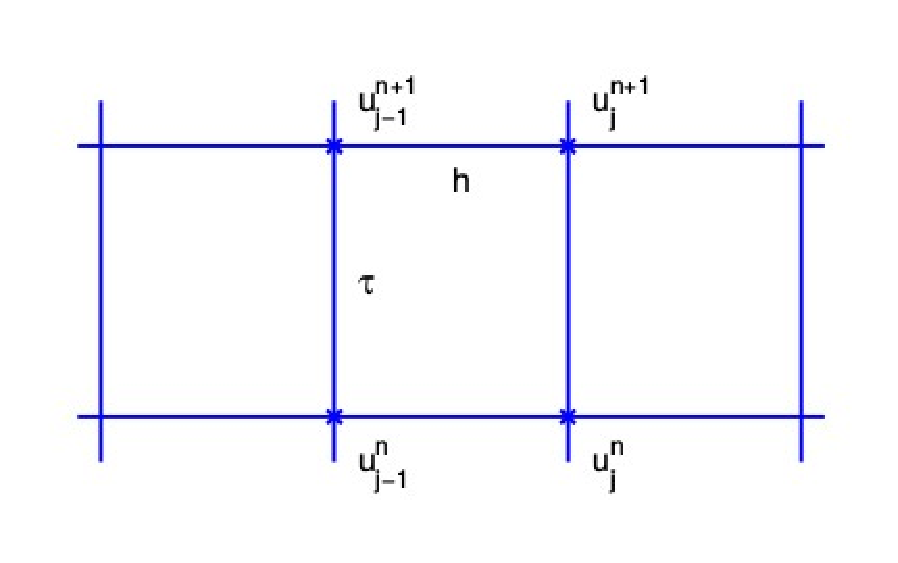
\includegraphics[height=4cm]{Figures/RCTFPM_mesh.eps}\\
	\caption[RCTFPM imaginary part]{}
\end{figure}



\begin{align*}
 u_{j}^{n+1} = \alpha_{-1}u_{j-1}^{n+1} + \beta_{-1}u_{j-1}^{n} + \beta_{0}u_{j}^{n}
\end{align*}

We expect the scheme to hold exactly for all the wave-formed functions in space.

\begin{align}
 V = {\{} v(x,t)|v(x,t) =  c_{1} + c_{2}\text{ exp}(ik_{j}(at-x)) + c_{3}\text{ exp}(-ik_{j}(at-x)), \hspace{0.5cm} \forall c_{1}, c_{2}, c_{3} \in \mathbb{C} {\}}  
\end{align}

where $k_{j}$ is the wave number in the j-th $[x_{j},x_{j+1}]$ cell and 'i' is the imaginary unit.
The complex-valued initial condition is denoted by $u_{0}(x)$. In the most general form it can be written as,
$u_{0}(x) = A_{0}(x)\text{exp}(iS_{0}(x))$, where $A_{0}(x)$ and $S_{0}(x)$ are real-valued functions.


We take the wave number as $k_{j} = S^{'}_{0}(x_{j})$ in each cell.

Taking the wave functions of $(c_{1}, c_{2}, c_{3}) = (1,0,0), (0,1,0), (0,0,1)$ in gives


\[ \begin{cases} 
      1 = \alpha_{-1} + \beta_{-1} + \beta_{0} \\
      \cos(k_{j}a\tau) = \alpha_{-1}\cos(k_{j}(a\tau+h)) +\beta_{-1} + \beta_{0}\\
      \sin(k_{j}a\tau) =  \alpha_{-1}\sin(k_{j}(a\tau+h)) - \beta_{-1}\sin(k_{j}h)\\
   \end{cases}
\]

By solving the above system we get,

\begin{align*}
 \alpha_{-1} &= \frac{\sin(k_{j}(a\tau-h)/2)}{\sin(k_{j}(a\tau+h)/2)}\\
 \beta_{-1} &= 1\\
 \beta_{0} &= -\alpha_{-1}
\end{align*}

\subsection{Stability Analysis}
We perform the Von Neumann Stability Analysis to get the stability criterion.
We susbtitute $u_{j}^{n}=e^{ij\xi h}$ and $u_{j}^{n+1} = G e^{ij\xi h}$ where G is the growth factor.
For the scheme to be stable we require
\begin{align*}
 |G| \leq 1
\end{align*}
Substituting in the scheme we get
\begin{align*}
 G e^{ij\xi h} &= \alpha_{-1}G e^{i(j-1)\xi h}+\beta_{-1} e^{i(j-1)\xi h}+\beta_{0} e^{ij\xi h}\\
 G &= \alpha_{-1}G e^{-i \xi h}+ e^{-i \xi h}-\alpha_{-1} \\
 (1-\alpha_{-1} e^{-i \xi h})G &= e^{-i \xi h}-\alpha_{-1}\\
 G &= \frac{e^{-i \xi h}-\alpha_{-1}}{1-\alpha_{-1} e^{-i \xi h}}\\ 
 \text{Taking absolute on both sides}\\
 |G| &= \Bigg{\lvert} \frac{e^{-i \xi h}-\alpha_{-1}}{1-\alpha_{-1} e^{-i \xi h}} \Bigg{\rvert}\\ \\
 |G| &= \frac{|e^{-i \xi h}-\alpha_{-1}|}{|1-\alpha_{-1} e^{-i \xi h}|}\\ \\
 |G| &= \frac{|\cos(\xi h) + i\sin(\xi h)-\alpha_{-1}|}{|1-\alpha_{-1} (\cos(\xi h) - i\sin(\xi h))|}\\ \\
 |G| &= \frac{|\cos(\xi h)-\alpha_{-1} + i\sin(\xi h)|}{|1-\alpha_{-1}\cos(\xi h) + i\alpha_{-1}\sin(\xi h)|}\\ \\
 |G| &= \sqrt{\frac{(\cos(\xi h)-\alpha_{-1})^2 + (\sin(\xi h))^2}{(1-\alpha_{-1}\cos(\xi h))^2 + (\alpha_{-1}\sin(\xi h))^2}}\\ \\
 |G| &= 1
\end{align*}
Thus the scheme is unconditionally stable.

This scheme is claimed to be second order in space.

\subsection{Example 1}
Consider the wave equation along with the given initial condition
\begin{align}
 \begin{split}
  u_{t} + u_{x} &= 0\\
   u(x,0) &= e^{-50x^2}e^{i\text{sin}(x)}
 \end{split} 
\end{align}
The analytical solution is given by
\begin{align}
 u(x,t) = e^{-50(x-t)^2}e^{i\text{sin}(x-t)}
\end{align}

The following plots and error estimates have been obtained on solving the above example using the tailored finite point method.\\

\begin{tabular}{|c|c|c|c|c|c|}
   \hline
   (h, $\tau$)  & (1/$2^{6}$,1/$2^{10}$)  & (1/$2^{7}$,1/$2^{10}$) & (1/$2^{8}$,1/$2^{10}$) &  (1/$2^{9}$,1/$2^{10}$)\\
  \hline
  Error  & 0.0293  & 0.0070 & 0.0016 &  0.0003\\
  \hline
  Order & -  &  2.05  & 2.08 & 2.32\\
\hline
\end{tabular}

\begin{figure}[htbp]
	\centering
		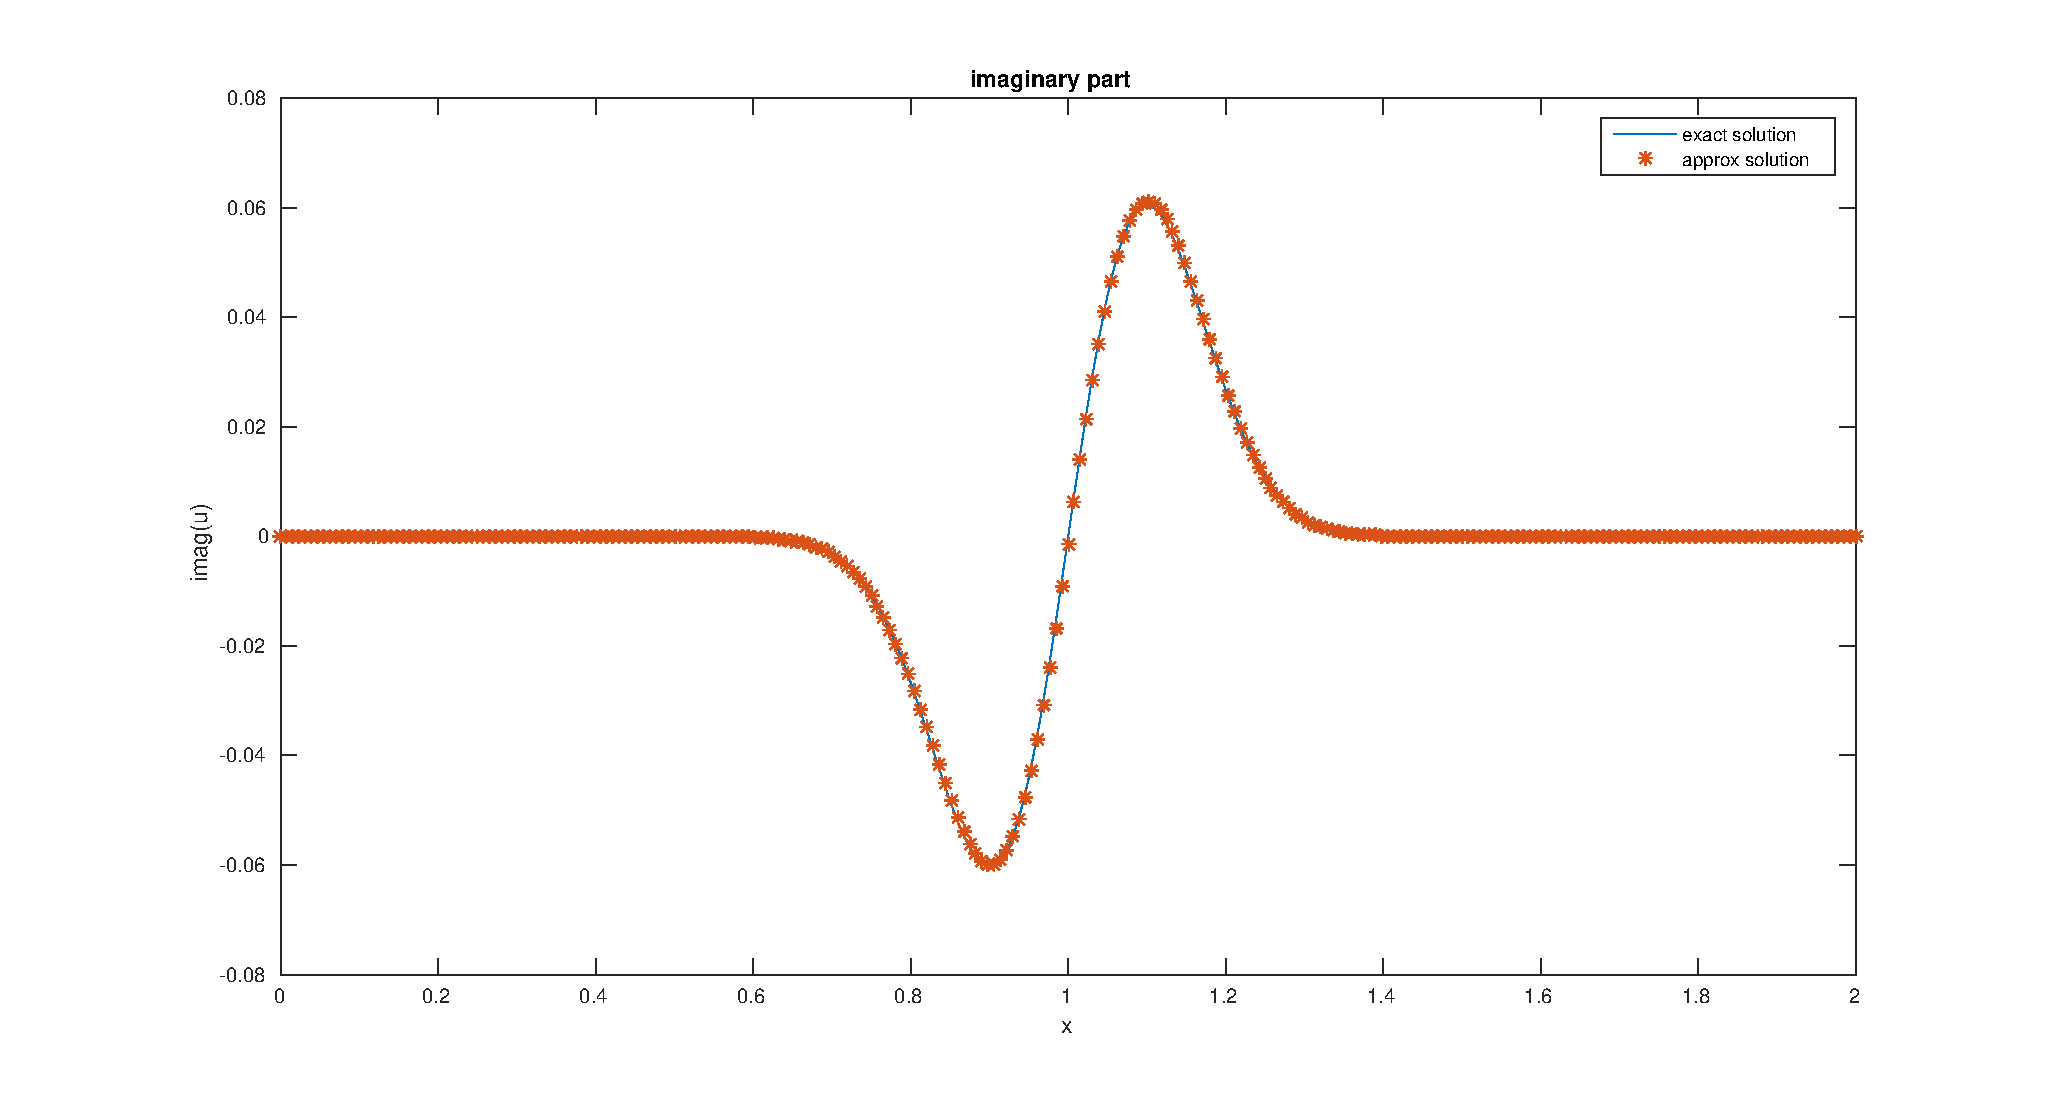
\includegraphics[height=8cm]{Figures/imag_RCTFPM2_2.eps}\\
		\rule{35em}{0.5pt}
	\caption[RCTFPM Real part]{}
\end{figure}

\begin{figure}[htbp]
	\centering
		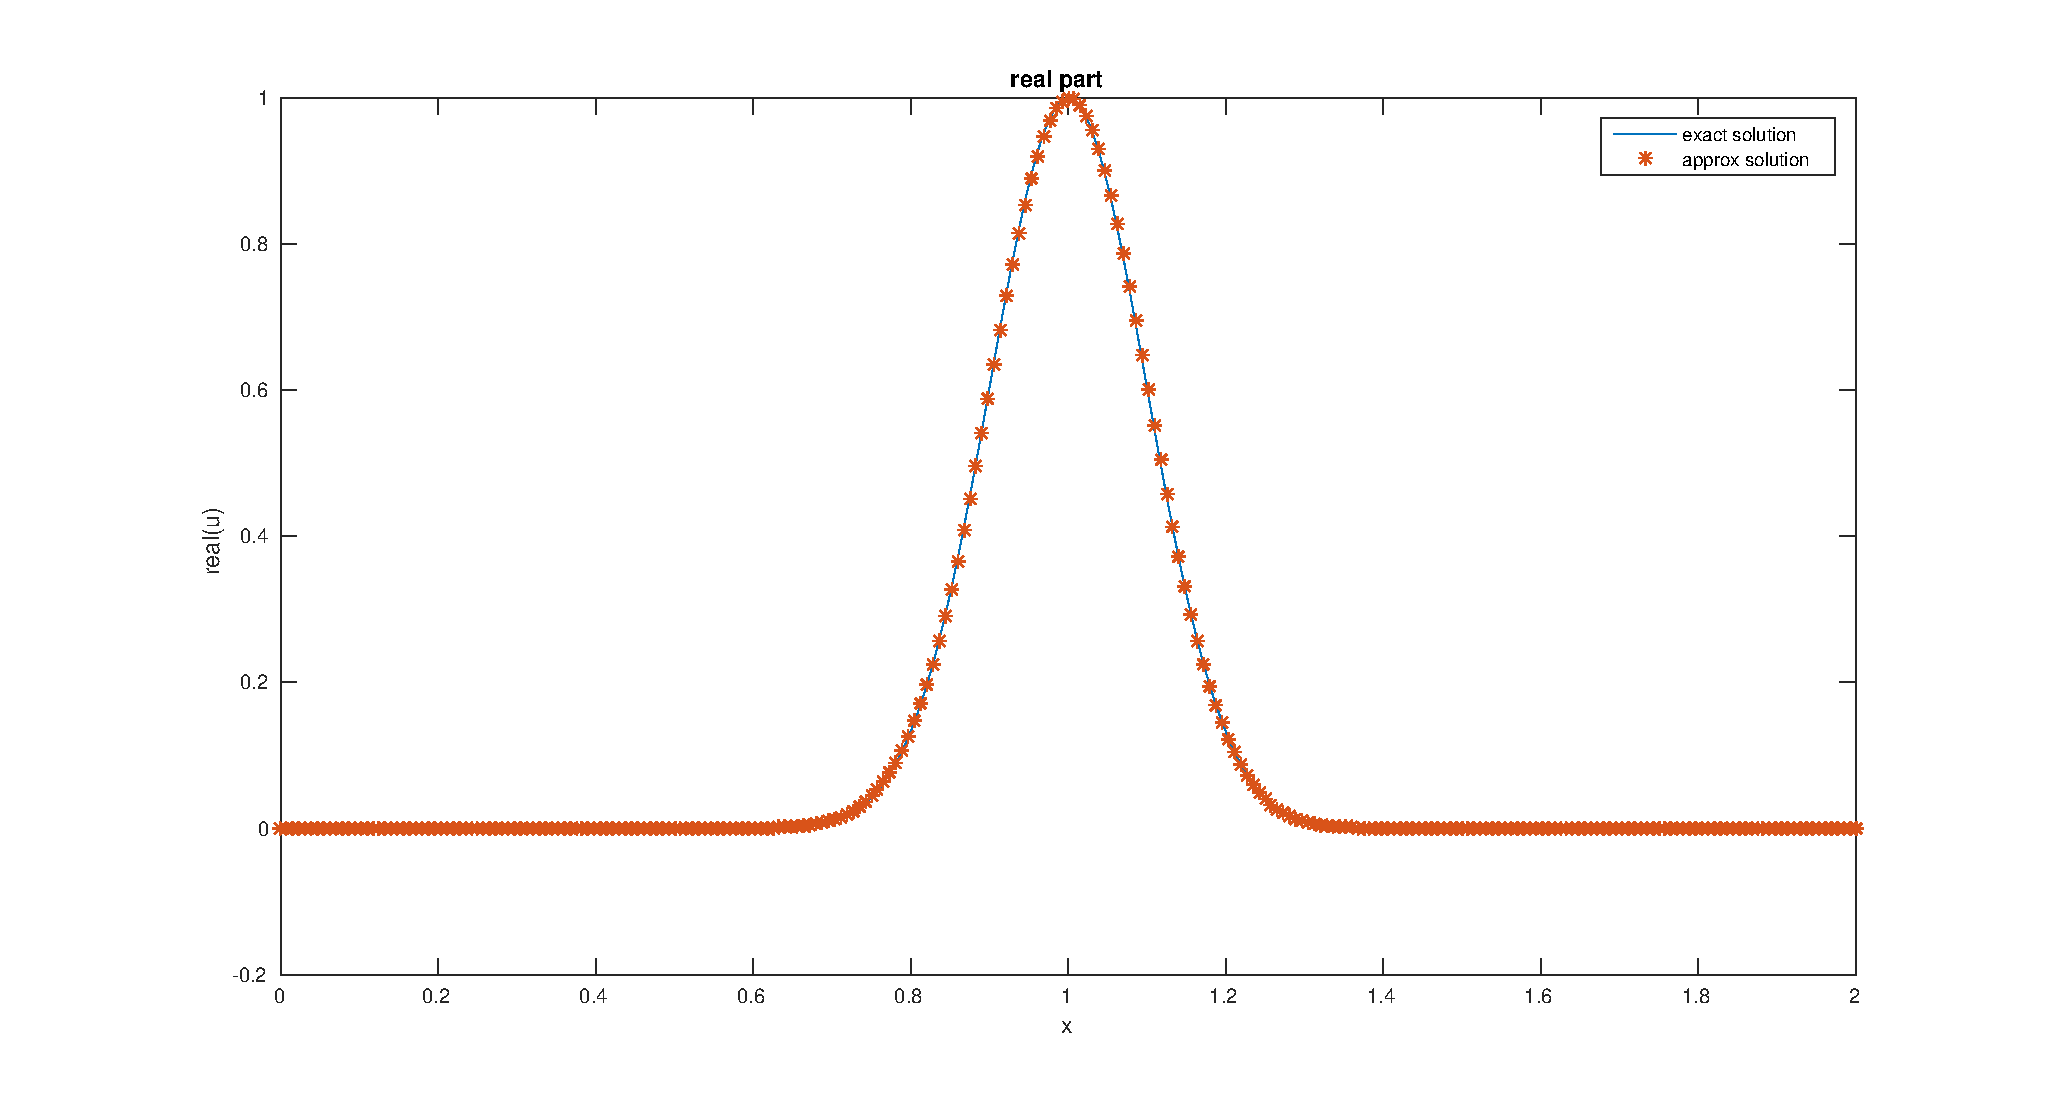
\includegraphics[height=8cm]{Figures/real_RCTFPM2_2.eps}\\
		\rule{35em}{0.5pt}
	\caption[RCTFPM imaginary part]{}
\end{figure}
\clearpage

\subsection{Example 2}
\begin{align}
 u_{t} + a(x)u_{x} = 0
\end{align}
The wave speed and initial condition are given as follows:
\begin{align}
 a(x) &= \pi + x\\
 u_{0}(x) &= e^{-50x^2}e^{i\sin(x)}
\end{align}
The exact solution is given by
\begin{align}
 u(x,t) = e^{-50((\pi+x)e^{-t}-\pi)^2}e^{(i\sin(\pi+x)e^{-t}-\pi)}
\end{align}
The wave number $k_{j}$ is taken to be $k_{j}=\cos(x_{j})$
Here we see that the wave speed is not a constant.
It is a linear function. The following approach is adopted when 'a' is not a constant:\\
We approximate $a(x)$ as
\begin{align}
 a(x) &\approx b_{j} + c_{j}x\hspace{5mm} \text{ where }\\
 b_{j} &= \frac{a(x_{j-1})x_{j}-a(x_{j})x_{j-1}}{h}
\end{align}
Then at the $n^{th}$ time step the solution can be locally approximated as
\begin{align}
 u(x_{j},t^{n}) = A_{0}(y_{j}^{n})e^{(iS_{0}(y_{j}^{n})/\epsilon)}
\end{align}
where
\begin{align}
 y_{j}^{n} = ((b_{j}+c_{j}x_{j})e^{-c_{j}t^{n}} -b_{j})/c_{j} 
\end{align}
We take the wave number as follows
\begin{align}
 k_{j}^{n} = S_{0}^{'}(y_{j}^{n})e^{-c_{n}t^{n}}/\epsilon
\end{align}

This example has been solved using the RCTFPM method. The following are the expressions for the coeffecients
\begin{align}
 \alpha_{-1}^{n} &= \frac{\sin(k_{j}^{n}(a_{j}\tau - h)/2)}{\sin(k_{j}^{n}(a_{j}\tau + h)/2)}\\
 \beta_{-1}^{n} &= 1\\
 \beta_{0}^{n} &= -\alpha_{-1}^{n}
\end{align}

The error estimates and plots obtained are given as follows:

\begin{tabular}{|c|c|c|c|c|c|}
   \hline
   (h, $\tau$)  & (1/$2^{6}$,1/$2^{10}$)  & (1/$2^{7}$,1/$2^{10}$) & (1/$2^{8}$,1/$2^{10}$) &  (1/$2^{9}$,1/$2^{10}$)\\
  \hline
  Error  & 0.0178  & 0.0058 & 0.0018 &  0.0007\\
  \hline
  Order & -  &  1.608  & 1.623 & 1.405\\
\hline
\end{tabular}

\begin{figure}[htbp]
	\centering
		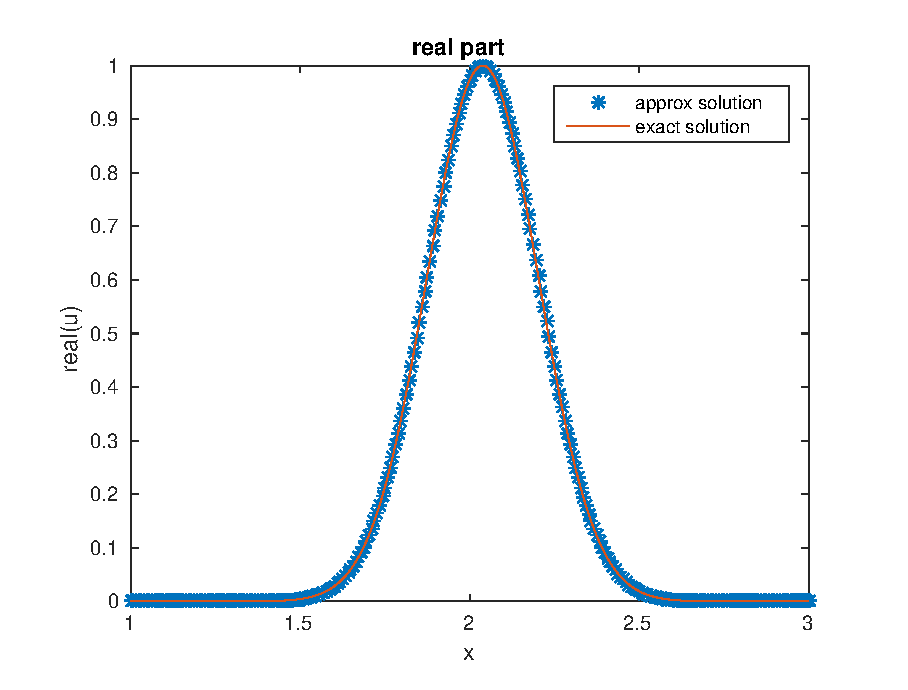
\includegraphics[height=8cm]{Figures/real_RCTFPM3_1.eps}\\
		\rule{35em}{0.5pt}
	\caption[RCTFPM Real part]{}
\end{figure}
\begin{figure}[htbp]
	\centering
		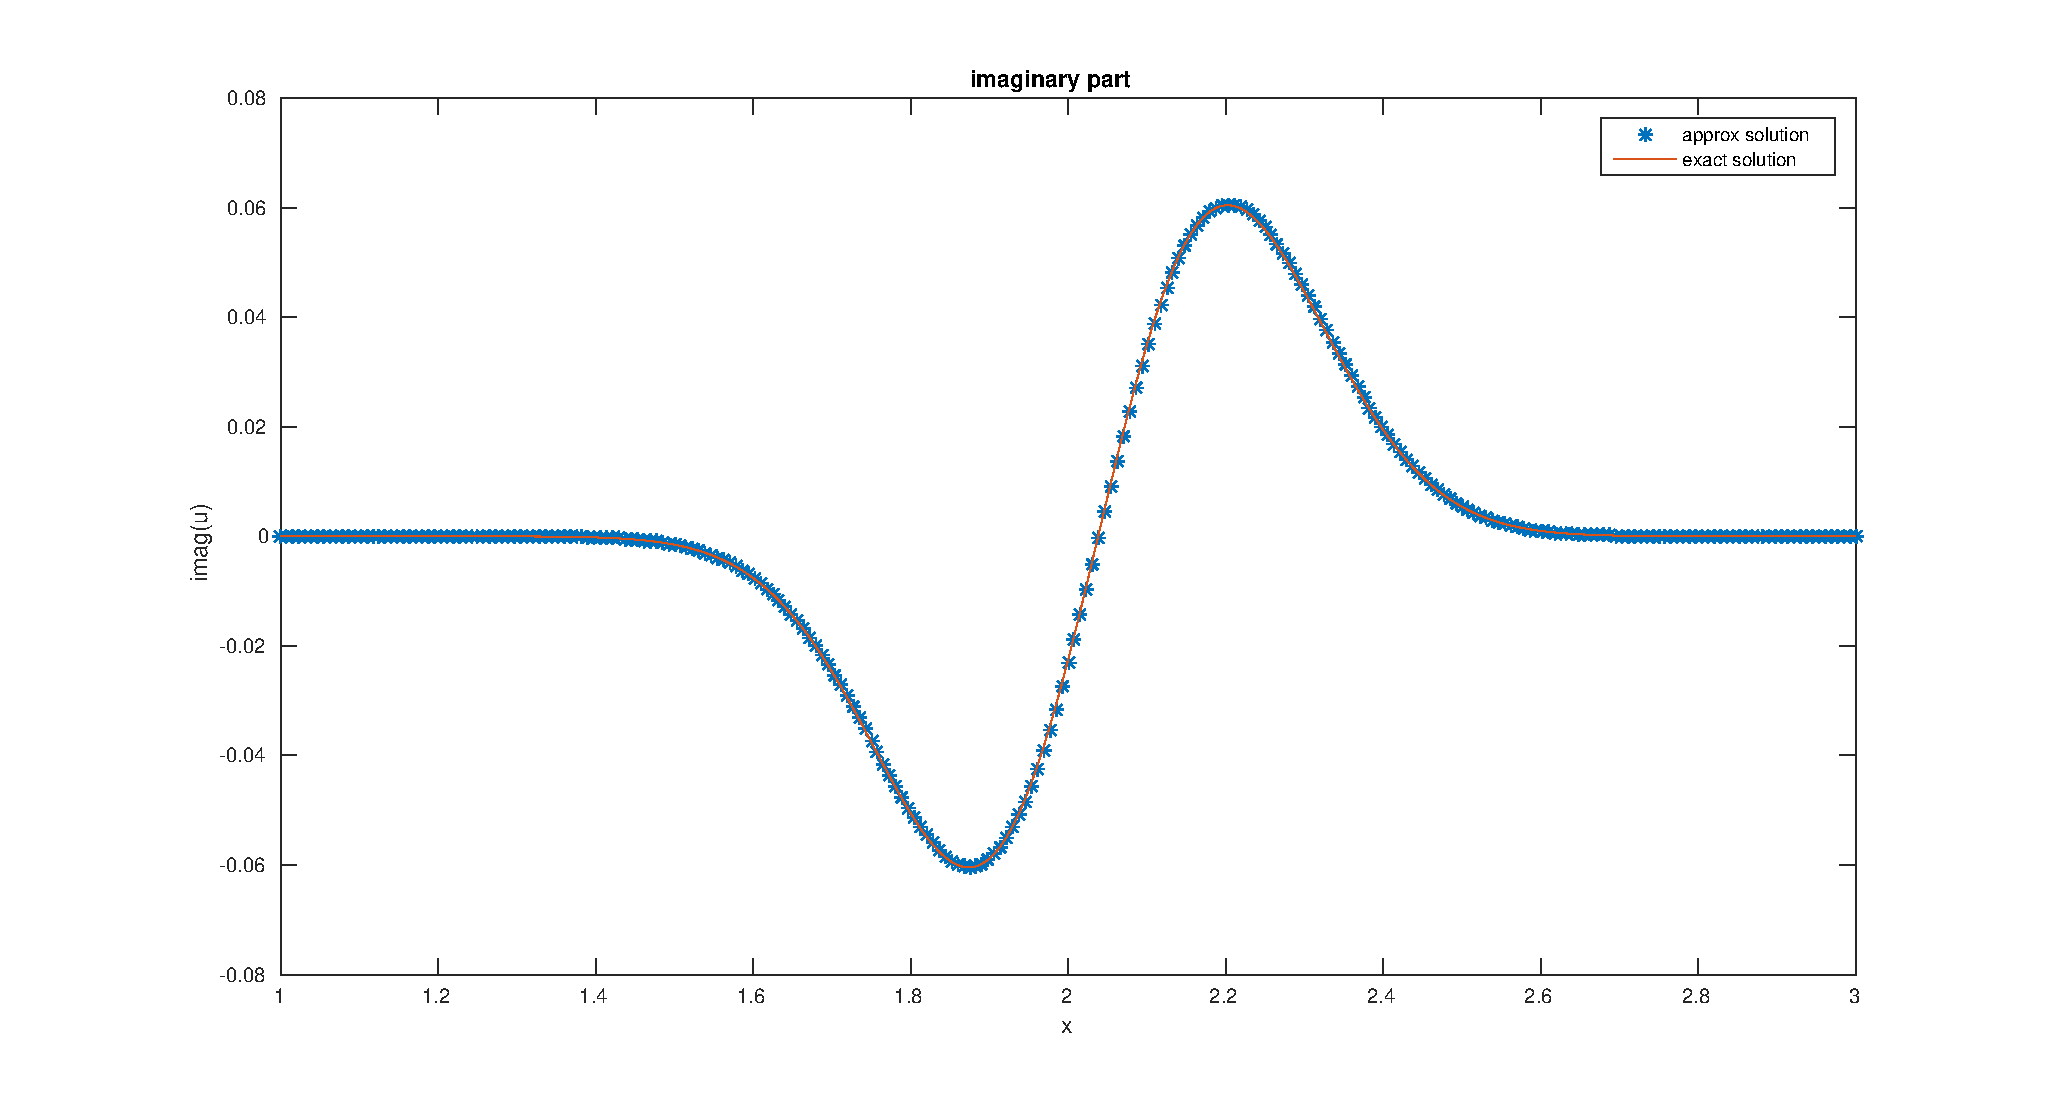
\includegraphics[height=8cm]{Figures/imag_RCTFPM3_1.eps}\\
		\rule{35em}{0.5pt}
	\caption[RCTFPM Real part]{}
\end{figure}
\clearpage
\subsection{Example 3}
\begin{align}
 u_{t} + a(x)u_{x} = 0
\end{align}
The wave speed and initial condition are given as follows:
\begin{align}
 a(x) &= 0.5 + x\\
 u_{0}(x) &= e^{-200x^2}e^{i\sin(x)/\epsilon}
\end{align}
The exact solution is given by
\begin{align}
 u(x,t) = e^{-50((\pi+x)e^{-t}-\pi)^2}e^{(i\sin(\pi+x)e^{-t}-\pi)}
\end{align}
The wave number $k_{j}$ is taken to be $k_{j}=\cos(x_{j})$

This example has been solved using the RCTFPM method.
The error estimates and plots obtained are given as follows:

\begin{tabular}{|c|c|c|c|c|c|}
   \hline
   (h, $\tau$)  & (1/$2^{7}$,1/$2^{6}$)  & (1/$2^{8}$,1/$2^{6}$) & (1/$2^{9}$,1/$2^{6}$) &  (1/$2^{10}$,1/$2^{6}$)\\
  \hline
  Error  & 0.0816  & 0.0381 & 0.0204 &  0.0105\\
  \hline
  Order & -  &  1.088  & 0.9102 & 0.9588\\
\hline
\end{tabular}

\begin{figure}[htbp]
	\centering
		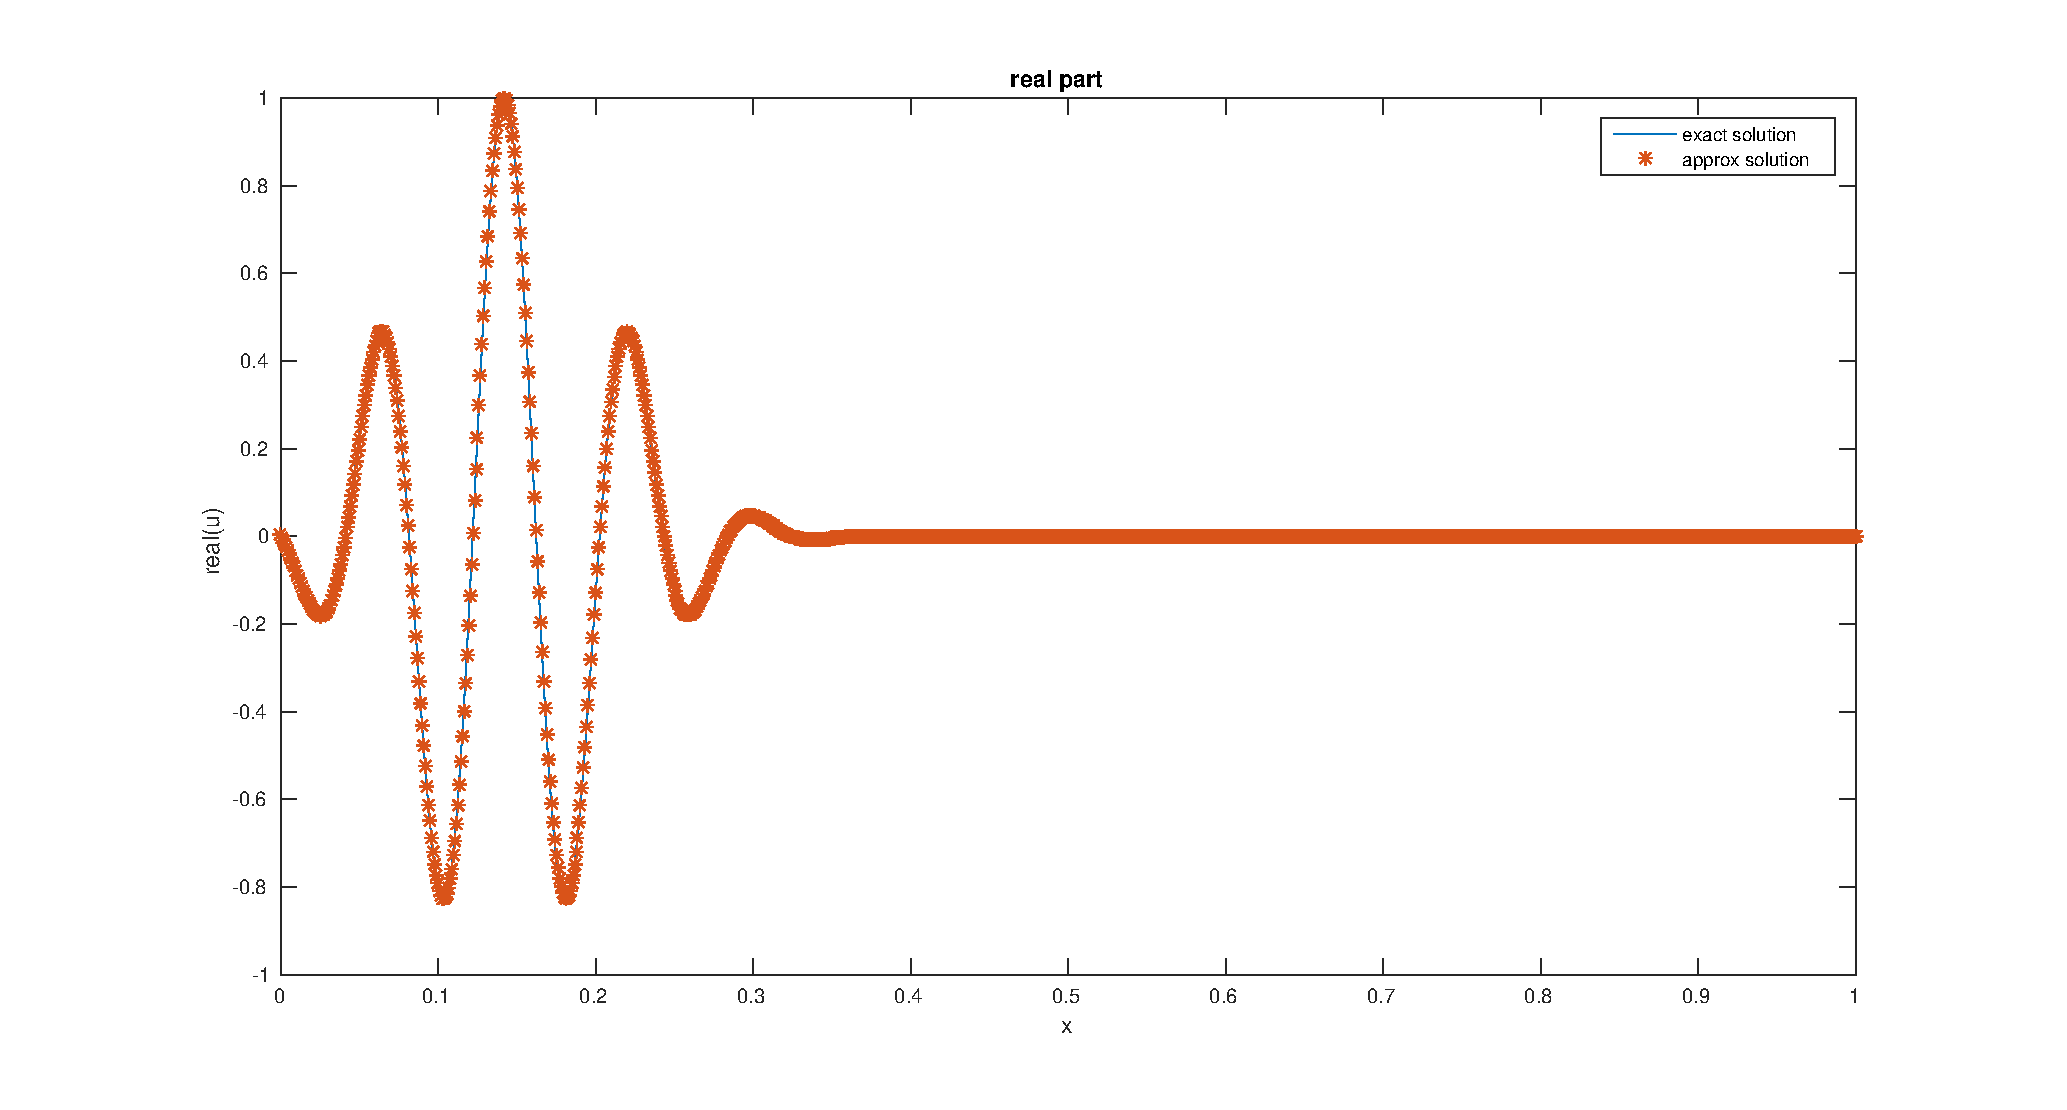
\includegraphics[height=8cm]{Figures/real_RCTFPM3_2.eps}\\
		\rule{35em}{0.5pt}
	\caption[RCTFPM Real part]{}
\end{figure}
\begin{figure}[htbp]
	\centering
		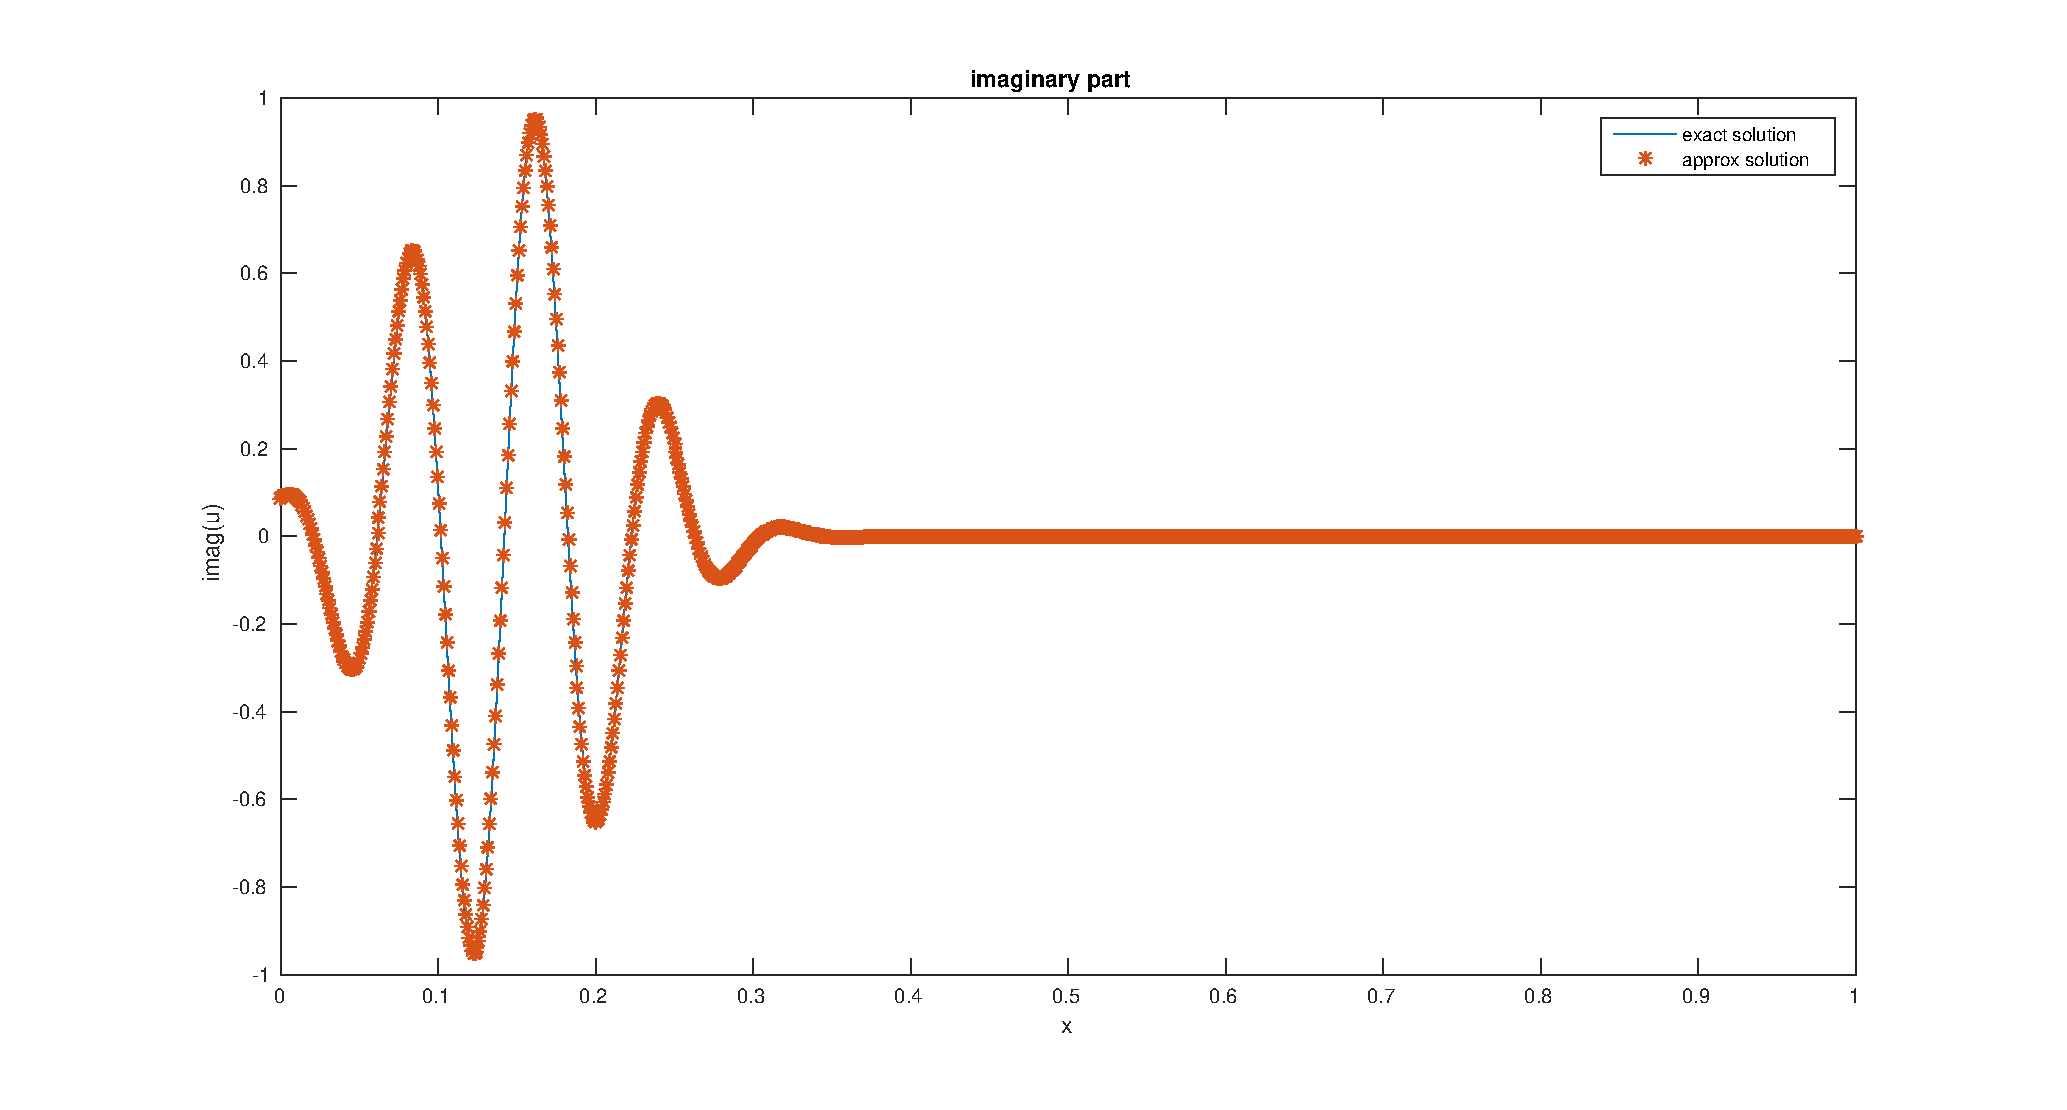
\includegraphics[height=8cm]{Figures/imag_RCTFPM3_2.eps}\\
		\rule{35em}{0.5pt}
	\caption[RCTFPM Real part]{}
\end{figure}
\clearpage

\section{Centered tailored finite point method (CTFPM)}
\begin{figure}[htbp]
	\centering
		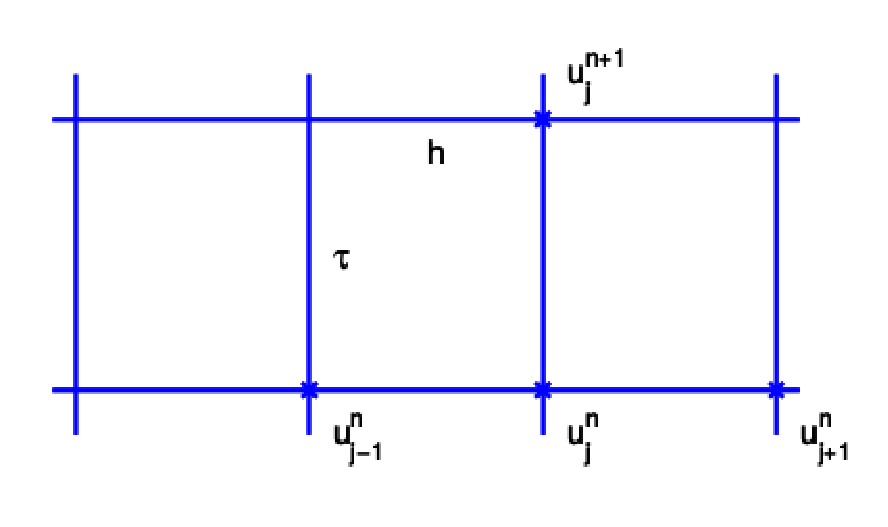
\includegraphics[height=4cm]{Figures/CTFPM_mesh.eps}\\
	\caption[RCTFPM imaginary part]{}
\end{figure}
We derive an explicit scheme as follows:

\begin{align}
u_{j}^{n+1} = \alpha_{-1}u_{j-1}^{n}+\alpha_{0}u_{j}^{n} + \alpha_{1}u_{j+1}^{n} 
\end{align}

The coefficients are taken as $(c_1,c_2,c_3) = (1,0,0),(0,1,0),(0,0,1)$ which gives us

\[ \begin{cases} 
      1 = \alpha_{-1} + \alpha_{0} + \alpha_{1} \\
      \cos(k_{j}a\tau) = \alpha_{-1}\cos(k_{j}h) +\alpha_{0} + \alpha_{1}\cos(k_{j}h)\\
      \sin(k_{j}a\tau) =  \alpha_{-1}\sin(k_{j}h) - \alpha_{1}\sin(k_{j}h)
   \end{cases}
\]

Solving this system yields,

\begin{align*}
 \alpha_{-1} =& \frac{\sin(k_{j}a\tau/2)\sin(k_{j}(a\tau + h)/2)}{\sin(k_{j}h/2)\sin(k_{j}h)}\\
 \alpha_{1} =& \frac{\sin(k_{j}a\tau/2)\sin(k_{j}(a\tau - h)/2)}{\sin(k_{j}h/2)\sin(k_{j}h)}\\
 \alpha_{0} =& 1 - \alpha{1} - \alpha_{-1}
\end{align*}

\subsection{Stability Analysis}
We perform the Von Neumann Stability Analysis to get the stability criterion.
Similar to the RCTFPM method we get,
\begin{align*}
 G = \alpha_{-1}e^{-i \xi h} + \alpha_{0} + \alpha_{1}e^{i \xi h}
\end{align*}
After calculating, the condition $|G| \leq 1$ is the same as
\begin{align*}
 1-\cos^2(k_{j}h)-\cos(k_{j}h) + \cos(k_{j} a \tau) + \cos(\xi h) - \cos(k_{j} h)\cos(k_{j} a \tau ) \cos(\xi h) \geq 0 \\
 (1+\cos(\xi h))(1-\cos(k_{j} h) \cos(k_{j} a \tau)) + (1+ \cos(k_{j} h))(\cos(k_{j} a \tau) - \cos(k_{j} h)) \geq 0
\end{align*}
As $k_{j} a \tau, k_{j} h << 1$.
Thus for the scheme to be stable we require $a \tau \leq h$.\\

\subsection{Accuracy}
We use the taylor series expansion to see the accuracy of the scheme.
Consider the terms
\begin{align*}
 u_{j-1}^{n} &\approx u(x-h,t) \approx u(x,t)-hu_{x}(x,t) + \frac{h^2}{2}u_{xx}(x,t)+o(h^3)\\
 u_{j+1}^{n} &\approx u(x+h,t) \approx u(x,t)+hu_{x}(x,t) + \frac{h^2}{2}u_{xx}(x,t)+o(h^3)\\
 u_{j}^{n} &\approx u(x,t)
\end{align*}
Substituting the above expressions in the  L.H.S of (1.22). We get
\begin{align*}
 &=\alpha_{-1}(u(x,t)-hu_{x}(x,t) + \frac{h^2}{2}u_{xx}(x,t))+\alpha_{0}(u(x,t)) + \alpha_{1}( u(x,t)+hu_{x}(x,t) + \frac{h^2}{2}u_{xx}(x,t))\\
 &=(\alpha_{-1}+\alpha_{0}+\alpha_{1})u(x,t) + h(\alpha_{1}-\alpha_{-1})u_{x}(x,t)+\frac{h^2}{2}(\alpha_{1}+\alpha_{-1})u_{xx}(x,t)\\
 &=u(x,t)+h(\alpha_{1}-\alpha_{-1})u_{x}(x,t)+\frac{h^2}{2}(\alpha_{1}+\alpha_{-1})u_{xx}(x,t)
\end{align*}
In th discrete form
\begin{align*}
 &=u_{j}^{n}+h((\alpha_{1}-\alpha_{-1})\frac{(u_{j+1}^{n}-u_{j-1}^{n})}{2h})+\frac{h^2}{2}(\alpha_{1}+\alpha_{-1})\frac{u_{j-1}^{n}-2u_{j}^{n}+u_{j+1}^{n}}{h^2}
\end{align*}
From calculating we have
\begin{align*}
 \alpha_{1}-\alpha_{-1}&= -\frac{\sin(k_{j}a\tau)}{\sin(k_{j} h)}\\
 \alpha_{1}+\alpha_{-1}&= \frac{\sin^2((k_{j}a\tau)/2)}{\sin^2((k_{j} h)/2)}
\end{align*}
As $k_j a\tau $,\hspace{2mm} $k_{j}h <<1$. We have
\begin{align*}
 \alpha_{1}-\alpha_{-1}&= -\frac{a\tau}{h}\\
 \alpha_{1}+\alpha_{-1}&= \frac{(a\tau)^2}{h^2}
\end{align*}
Substituting above we get,
\begin{align*}
 &=u_{j}^{n}-\frac{(a\tau)}{2h} (u_{j+1}^{n}-u_{j-1}^{n})+\frac{(a\tau)^2}{2h^2} (u_{j-1}^{n}-2u_{j}^{n}+u_{j+1}^{n})
\end{align*}
Equating with R.H.S we get

\begin{align*}
 u_{j}^{n+1} = u_{j}^{n} - \frac{a \tau}{2h} (u_{j+1}^{n}-u_{j-1}^{n}) + (a \tau)^2\bigg{(}\frac{u_{j-1}^{n}-2u_{j}^{n}+u_{j+1}^{n}}{2h^2}\bigg{)}
\end{align*}

This is the Lax Wendroff scheme which is second order accurate.

This scheme is second order in space.


\subsection{Example}
Consider the wave equation along with the given initial condition
\begin{align}
 \begin{split}
  u_{t} + u_{x} &= 0\\
   u(x,0) &= e^{-50x^2}e^{i\text{sin}(x)}
 \end{split} 
\end{align}
The analytical solution is given by
\begin{align}
 u(x,t) = e^{-50(x-t)^2}e^{i\text{sin}(x-t)}
\end{align}

The following plots and error estimates have been obtained on solving the above example using the tailored finite point method.\\

\vspace{2cm}

\begin{tabular}{|c|c|c|c|c|c|}
   \hline
   (h, $\tau$)  & (1/$2^{6}$,1/$2^{7}$)  & (1/$2^{7}$,1/$2^{8}$) & (1/$2^{8}$,1/$2^{9}$) &  (1/$2^{9}$,1/$2^{10}$)\\
  \hline
  Error  & 0.03996  & 0.01049 & 0.00265 &  6.65558e-04\\
  \hline
  Order & -  &  1.92  & 1.98 & 1.99\\
\hline
\end{tabular}

\begin{figure}[htbp]
	\centering
		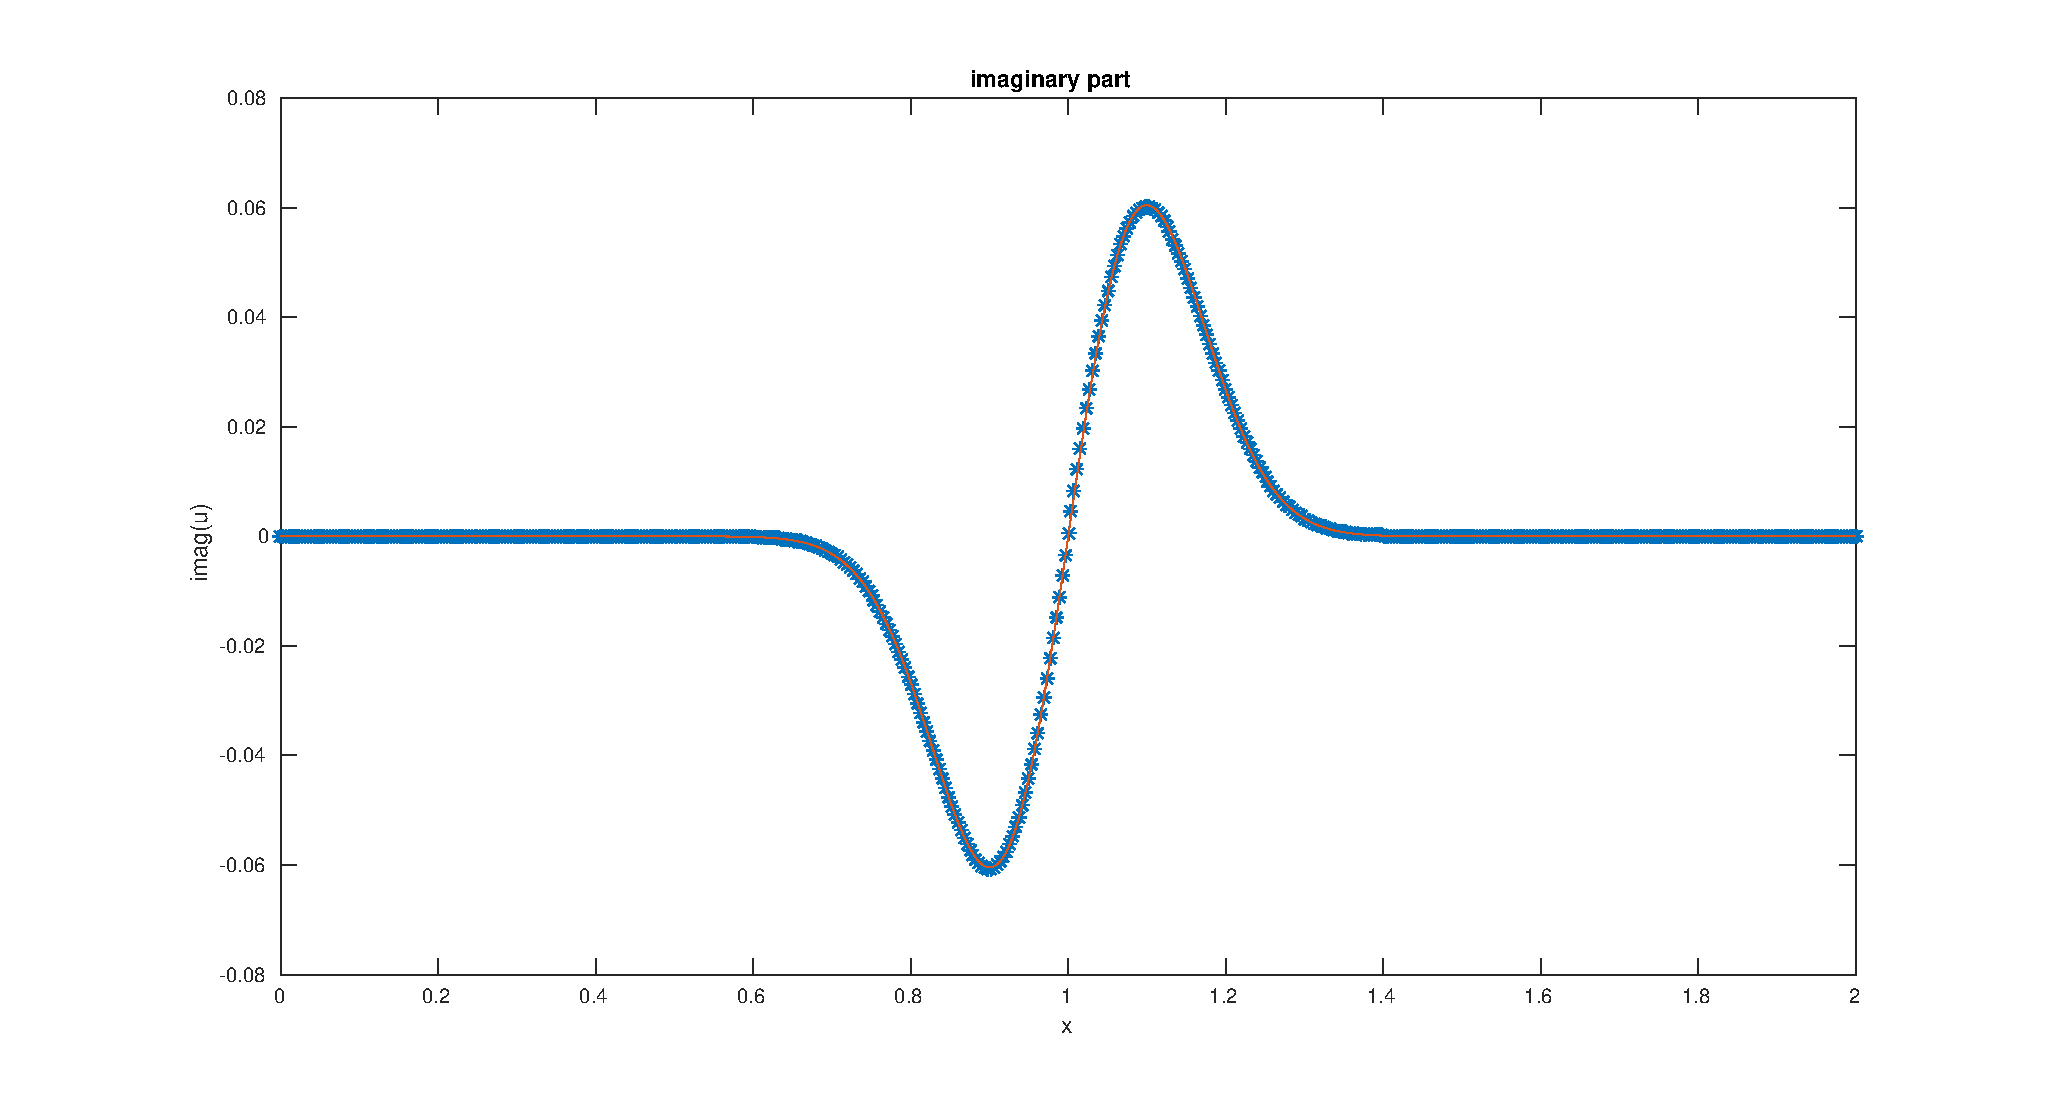
\includegraphics[height=8cm]{Figures/imag_CTFPM.eps}\\
		\rule{35em}{0.5pt}
	\caption[RCTFPM Real part]{}
\end{figure}

\begin{figure}[htbp]
	\centering
		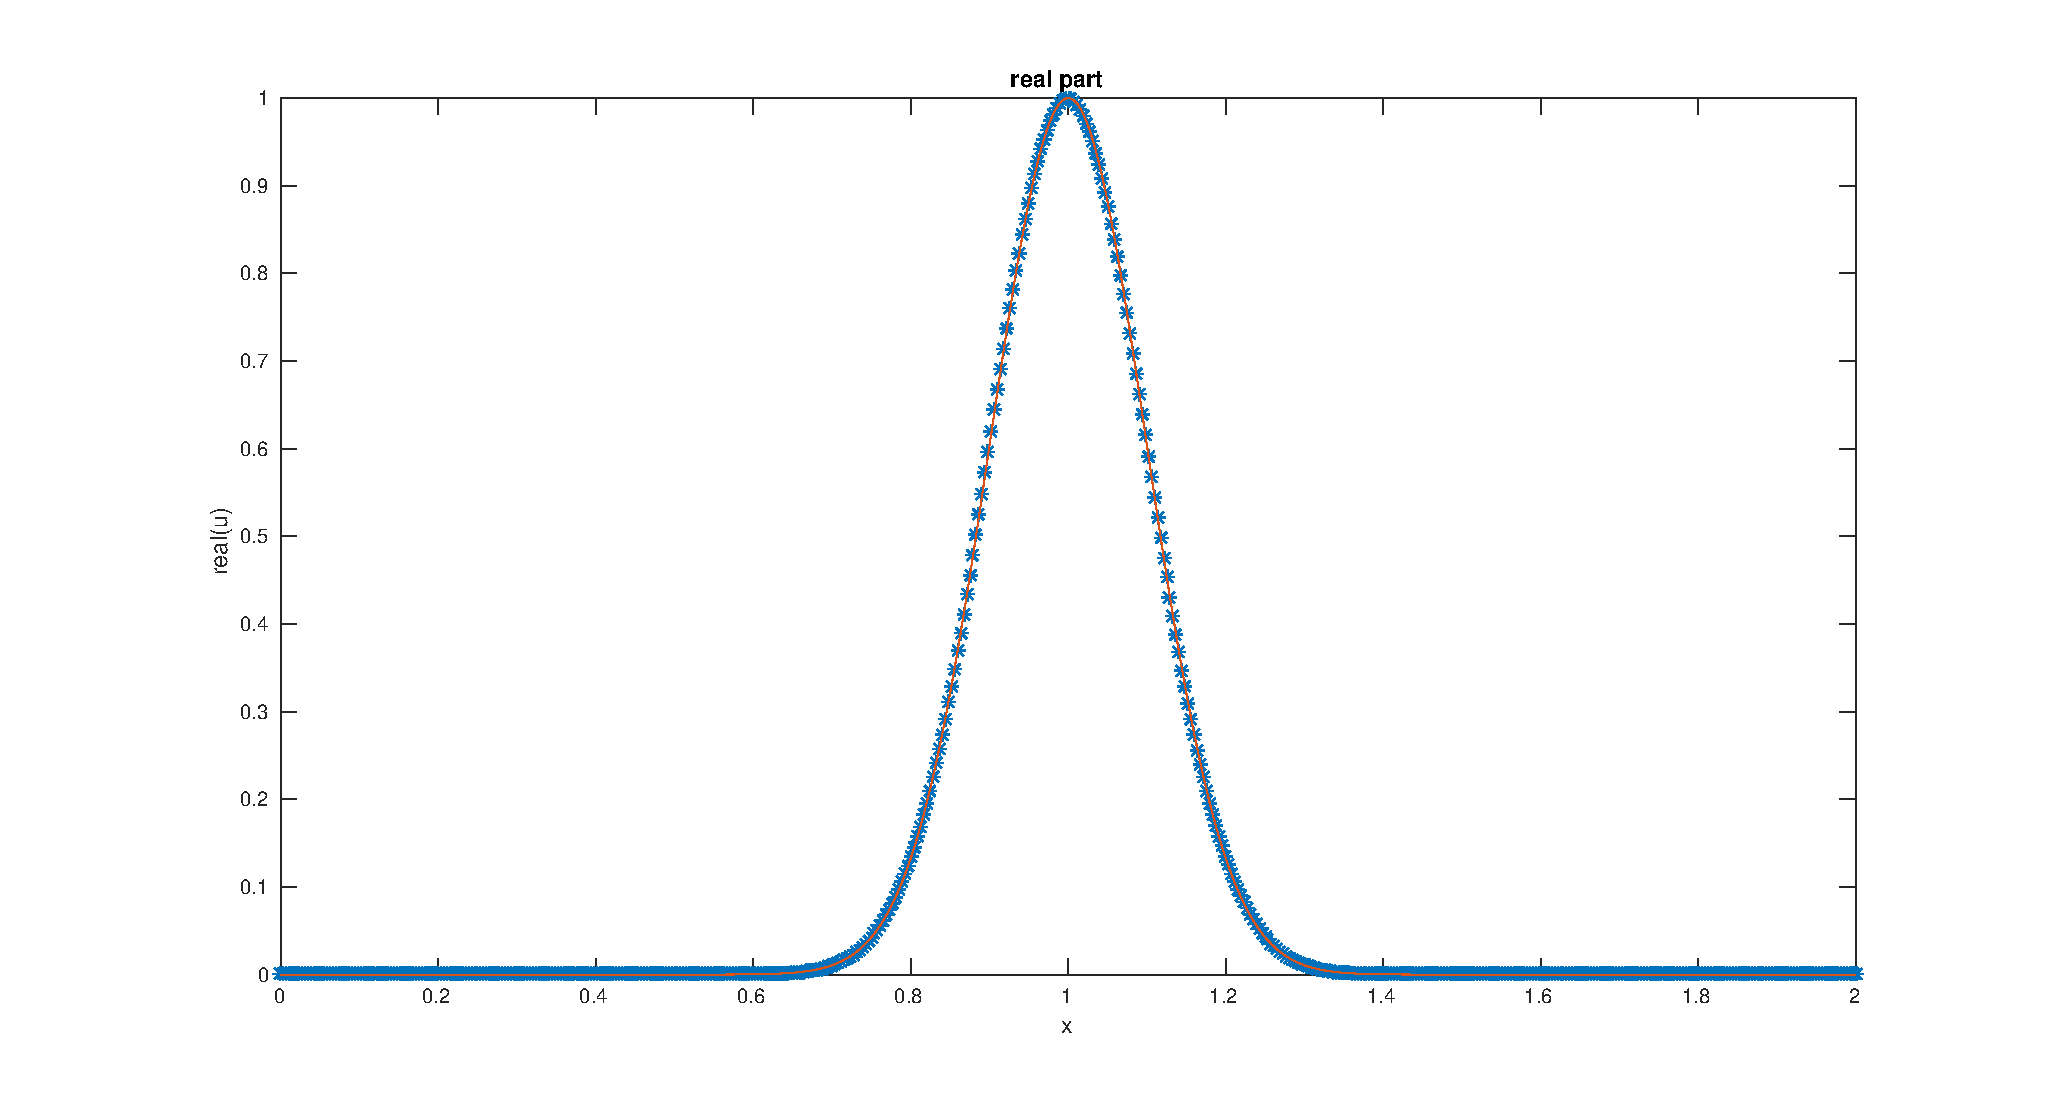
\includegraphics[height=8cm]{Figures/real_CTFPM.eps}\\
		\rule{35em}{0.5pt}
	\caption[RCTFPM imaginary part]{}
\end{figure}


\clearpage

\section{One Sided Tailored Finite Point Method (OSTFPM)}
\begin{figure}[htbp]
	\centering
		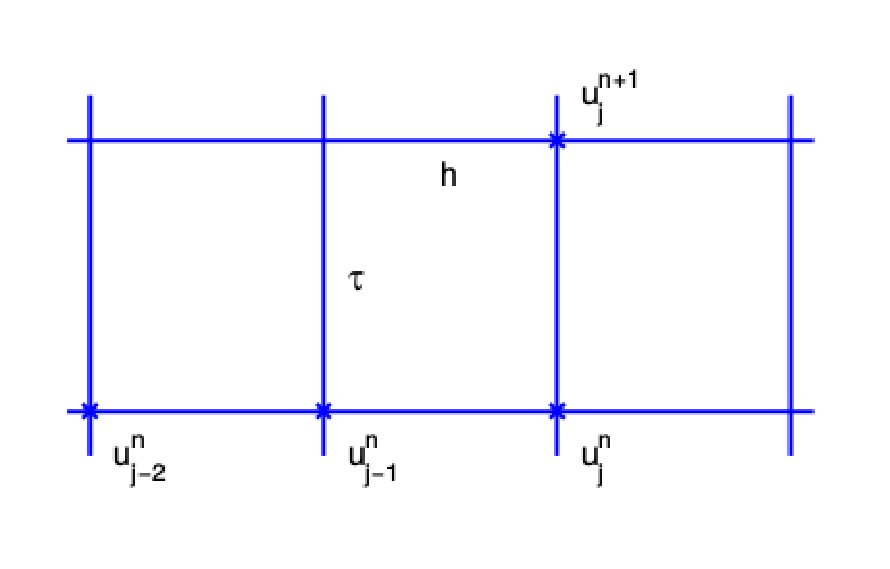
\includegraphics[height=4cm]{Figures/OSTFPM_mesh.eps}\\
	\caption[RCTFPM imaginary part]{}
\end{figure}
Many a times for boundary value problems the OSTFPM is an efficient method.The scheme is given as follows:
\begin{align}
 u_{j}^{n+1} = \alpha_{-2}u_{j-2}^{n} + \alpha_{-1}u_{j-1}^{n} + \alpha_{0}u_{j}^{n}
\end{align}

The coefficients are taken as $(c_1,c_2,c_3) = (1,0,0),(0,1,0),(0,0,1)$ which gives us

\[ \begin{cases} 
      1 = \alpha_{-2} + \alpha_{-1} + \alpha_{0} \\
      \cos(k_{j}a\tau) = \alpha_{-2}\cos(2k_{j}h) +\alpha_{-1}\cos(k_{j} h) + \alpha_{0}\\
      \sin(k_{j}a\tau) =  \alpha_{-2}\sin(2k_{j}h) + \alpha_{-1}\sin(k_{j}h)\\
   \end{cases}
\]
this gives us

\begin{align*}
 \alpha_{-2} &= \frac{\sin(k_{j}a\tau /2)\sin(k_{j}(a\tau - h)/2)}{\sin(k_{j}h/2)\sin(k_{j}h)}\\
 \alpha_{-1} &= \frac{\sin(k_{j}a\tau /2)\sin(k_{j}(a\tau - 2h)/2)}{\sin^2(k_{j}h/2)}\\
 \alpha_{0} &= 1-\alpha_{-2}-\alpha_{-1}
\end{align*}

\subsection{Stability Criterion}
%We perform the Von Neumann Stability Analysis to get the stability criterion.
The stability criterion of the scheme is a better than CTFPM. For the scheme to be stable we require
$\tau \leq 2h $.\\
%\begin{align*}
% G e^{i j \xi h} &= \alpha_{-2} e^{i (j-2) \xi h} + \alpha_{-1}e^{i (j-1) \xi h} + \alpha_{0}e^{i j \xi h}\\
% G &= \alpha_{-2} e^{-2 i \xi h} + \alpha_{-1} e^{-i \xi h} + \alpha_{0}
%\end{align*}
%On solving the above equation we require $a \tau \leq 2h$ for the scheme to be stable.
This scheme is second order in space.

\subsection{Accuracy}
\begin{align*}
 & u_{j-2}^{n} \approx u(x-2,t) \approx u(x,t) - 2h u_{x}(x,t) +2h^2 u_{xx}(x,t) + o(h^3)\\
 & u_{j-1}^{n} \approx u(x-1,t) \approx u(x,t) -h u_{x} + \frac{h^2}{2} u_{xx}(x,t) +o(h^3)\\
 & u_{j}^{n} \approx u(x,t)
\end{align*}

Substituting these values in the scheme, we get
\begin{align*}
 &= \alpha_{-2}(u-2hu_{x}+2h^2u_{xx}) + \alpha_{-1}(u-hu_{x}+\frac{h^2}{2}) + \alpha_{0}u_{j}^{n}\\
 &= (\alpha_{-2}+\alpha_{-1}+\alpha_{0})u - h(2 \alpha_{-2} + \alpha_{-1})u_{x} + h^2(\frac{\alpha_{-1}}{2}+2 \alpha_{-2}) u_{xx}\\
 &= u - h(\alpha_{-2}+\alpha_{-1})u_{x} + h^2 (2 \alpha_{-2} + \alpha_{-1}/2) u_{xx}\\
 &= u-a\tau u_{x} + \frac{(a \tau)^2}{2}u_{xx}\\
\end{align*}

In discrete form

\begin{align*}
 u_{j}^{n} - \frac{a \tau}{2h} (u_{j+1}^{n}-u_{j-1}^{n}) + \frac{(a \tau)^2}{2}\bigg{(}\frac{u_{j-1}^{n}-2u_{j}^{n}+u_{j+1}^{n}}{h^2}\bigg{)}
\end{align*}
Equating with R.H.S we get

\begin{align*}
 u_{j}^{n+1} = u_{j}^{n} - \frac{a \tau}{2h} (u_{j+1}^{n}-u_{j-1}^{n}) + \frac{(a \tau)^2}{2h^2}(u_{j-1}^{n}-2u_{j}^{n}+u_{j+1}^{n})
\end{align*}

This is the Lax Wendroff scheme which is second order accurate.

\subsection{Example}
Consider the wave equation along with the given initial condition
\begin{align}
 \begin{split}
  u_{t} + u_{x} &= 0\\
   u(x,0) &= e^{-50x^2}e^{i\text{sin}(x)}
 \end{split} 
\end{align}
The analytical solution is given by
\begin{align}
 u(x,t) = e^{-50(x-t)^2}e^{i\text{sin}(x-t)}
\end{align}

The following plots and error estimates have been obtained on solving the above example using the tailored finite point method.\\

\begin{tabular}{|c|c|c|c|c|c|}
   \hline
   (h, $\tau$)  & (1/$2^{6}$,1/$2^{7}$)  & (1/$2^{7}$,1/$2^{8}$) & (1/$2^{8}$,1/$2^{9}$) &  (1/$2^{9}$,1/$2^{10}$)\\
  \hline
  Error  & 0.1203  & 0.0434 & 0.0153 &  0.0054\\
  \hline
  Order & -  &  1.47  & 1.50 & 1.49\\
\hline
\end{tabular}


\begin{figure}[htbp]
	\centering
		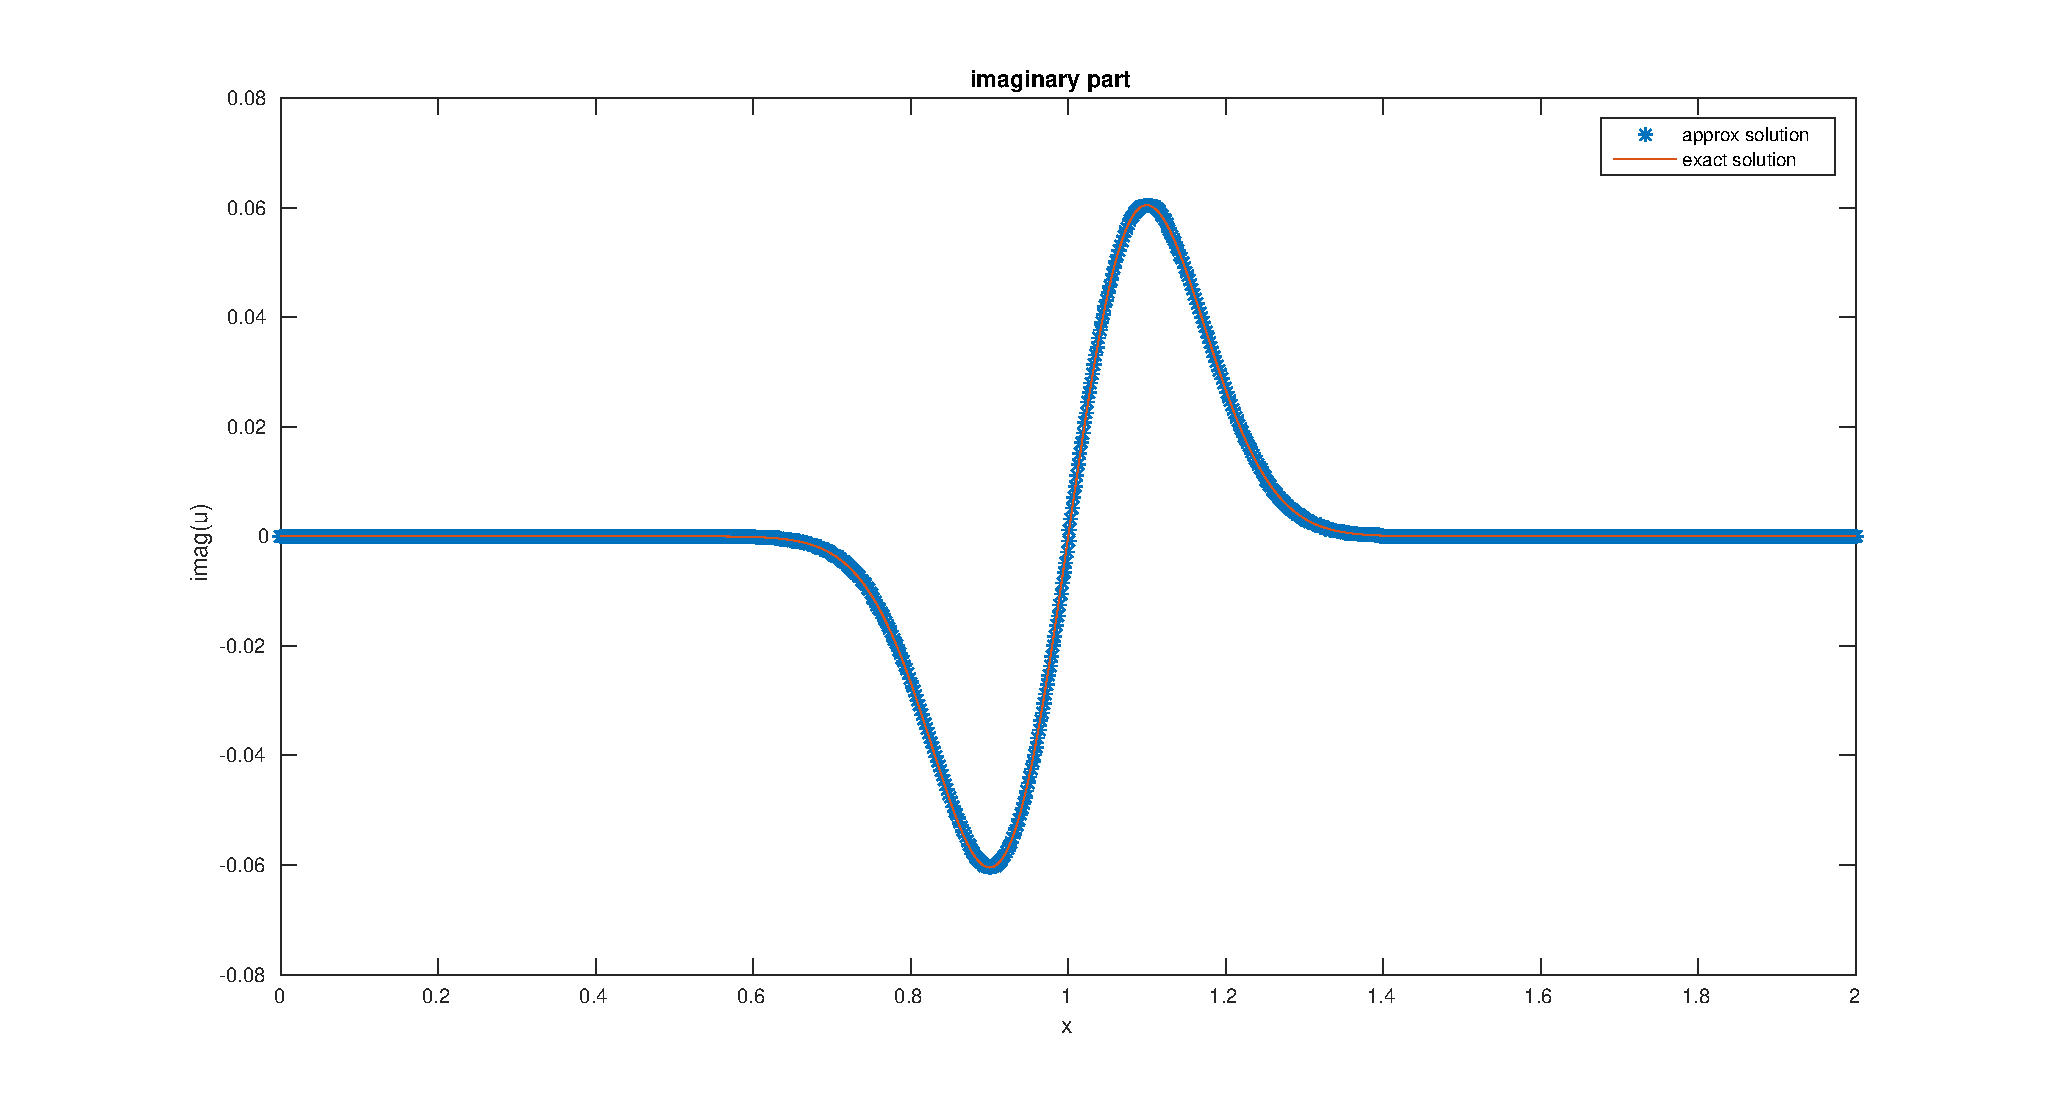
\includegraphics[height=8cm]{Figures/imag_OSTFPM_2_1.eps}\\
		\rule{35em}{0.5pt}
	\caption[OSTFPM imaginary part]{}
\end{figure}

\begin{figure}[htbp]
	\centering
		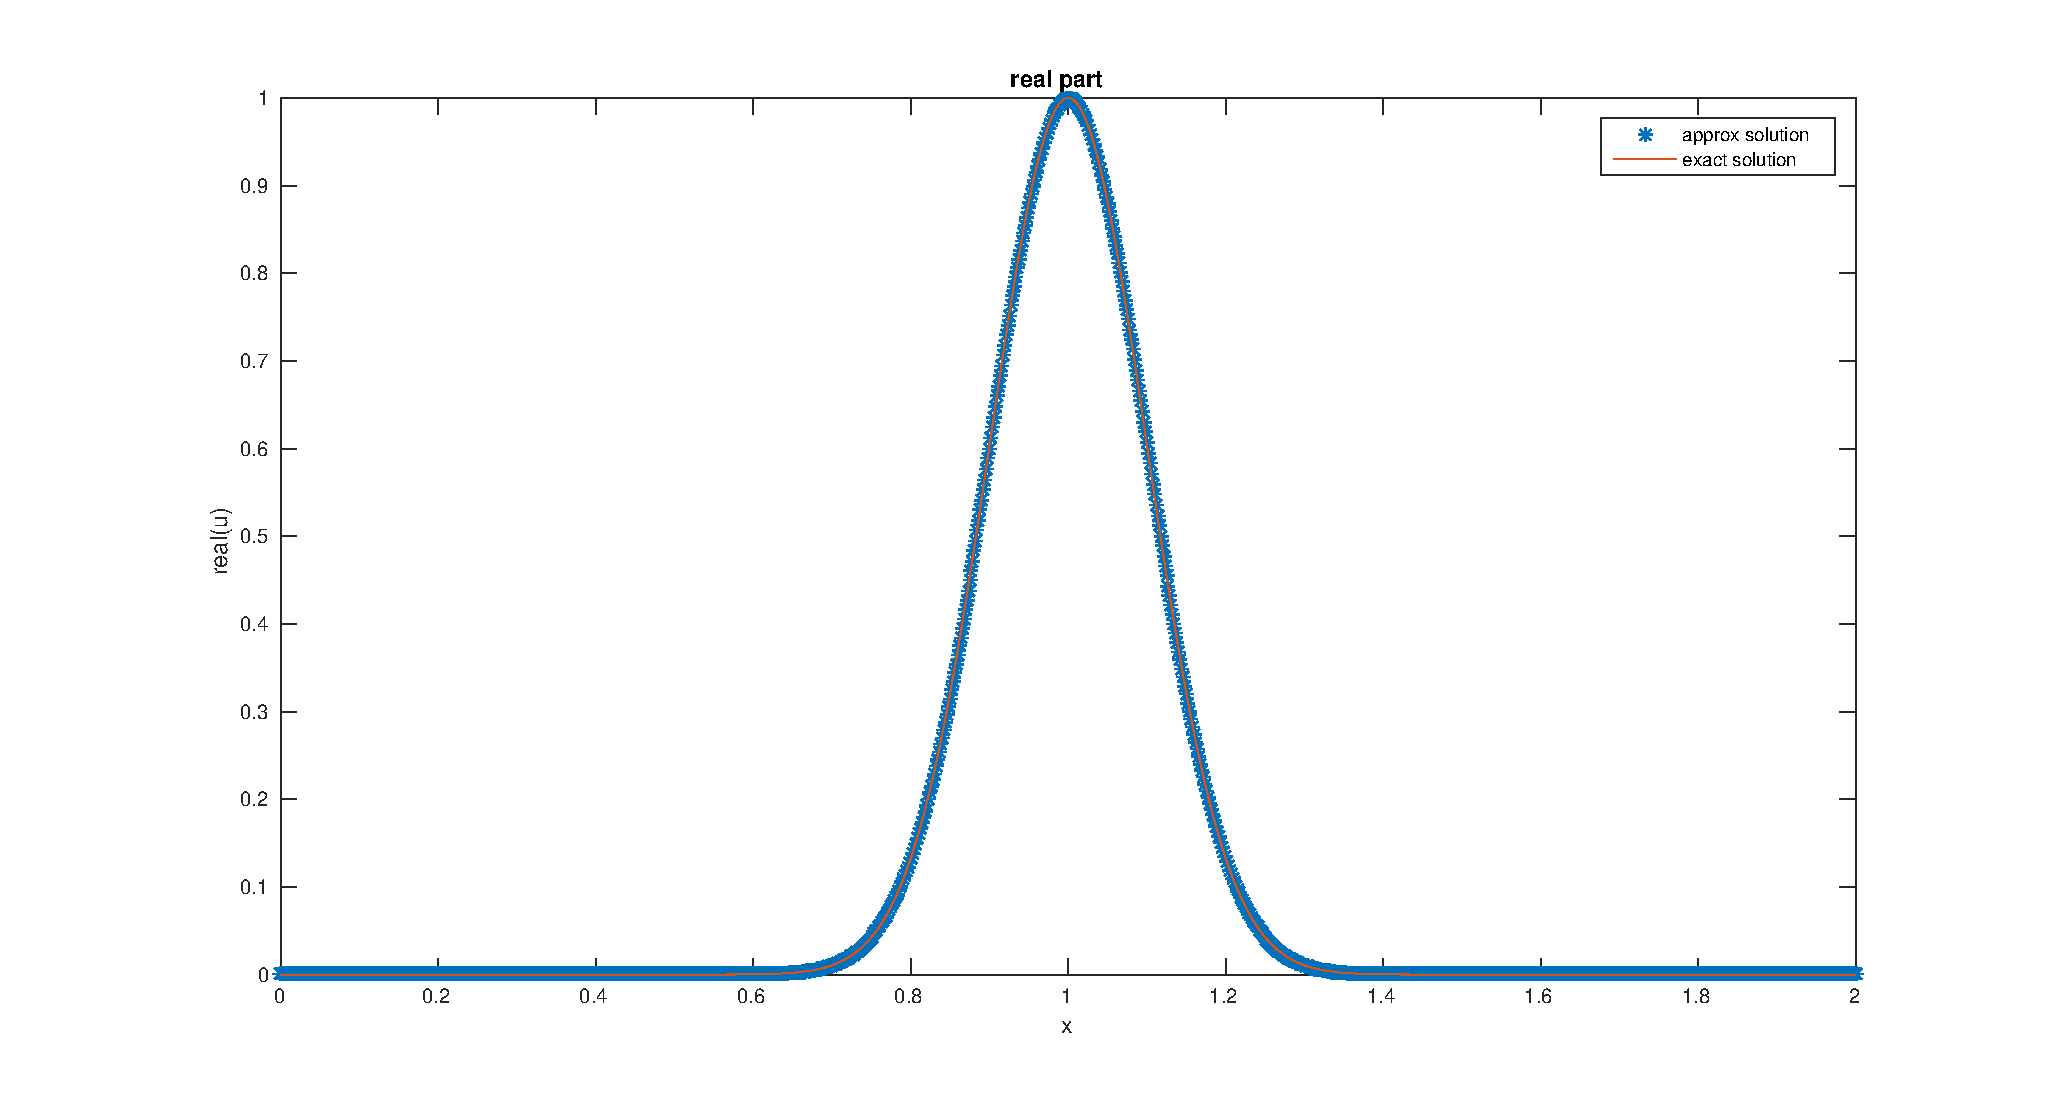
\includegraphics[height=8cm]{Figures/real_OSTFPM_2_1.eps}\\
		\rule{35em}{0.5pt}
	\caption[OSTFPM real part]{}
\end{figure}






% Chapter 1

\chapter{Parabolic Problem} % Main chapter title

\label{Chapter2} % For referencing the chapter elsewhere, use \ref{Chapter1} 

\lhead{Chapter 2. \emph{Parabolic and 2D Problem}} % This is for the header on each page - perhaps a shortened title

%----------------------------------------------------------------------------------------

\section{Parabolic Problem}
We consider the convection-diffusion-reaction equation with the following conditions
\begin{align}
 & u_{t}-\epsilon u_{xx} + bu_{x} + cu = f \text{ for } (x,t) \in \Omega=(0,1)\\
 & u(x,0) = \phi(x)\\
 & u(0,t) = \alpha(t), u(1,t) = \beta(t)
\end{align}
The coefficients on the grid points are approximated as follows:
\begin{align*}
 b(x,t) \approx b_{j}^{n}, \hspace{5mm} c(x,t) \approx c_{j}^{n}, \hspace{5mm}f(x,t) \approx f_{j}^{n} \text{ for } x \in [x_{j-1},x_{j+1}],\hspace{2mm} t \in [t^{n},t^{n+1}]
\end{align*}
Thus the equation is now,
\begin{align*}
 u_t -\epsilon u_{xx} + b_{j}^{n} + c_{j}^{n} = f_{j}^{n} \text{ for } x \in [x_{j-1},x_{j+1}],\hspace{2mm} t \in [t^{n},t^{n+1}]
\end{align*}
For $c_{j}^{n}>0$, we let $v(x,t) = u(x,t)-f_{j}^{n}/c_{j}^{n}$. Then $v(x,t)$ satisfies
\begin{align*}
 v_t-\epsilon v_{xx} + b_{j}^{n} + c_{j}^{n}v = 0 \text{ for } x \in [x_{j-1},x_{j+1}],\hspace{2mm} t \in [t^{n},t^{n+1}]
\end{align*}
Let
\begin{align*}
 H_{3} = \{ w(x,t) | = w(x,t) = \beta_{0}e^{-c_{j}^{n}t}, \beta_{1}e^{\lambda_{+}x},\beta_{2}e^{\lambda_{-}x} \text{ for } \beta_{i} \in R     \}
\end{align*}
with
\begin{align*}
 \lambda_{\pm} = \frac{b_{j}^{n}}{2\epsilon} \pm \sqrt{\frac{(b_{j}^{n})^2}{4 \epsilon^2}+\frac{c_{j}^{n}}{\epsilon}}
\end{align*}
We use the following scheme
\begin{align*}
 v_{j}^{n+1} = \alpha_{1}v_{j-1}^{n}+\alpha_{2}v_{j}^{n}+\alpha_{3}v_{j+1}^{n}
\end{align*}
Substituting the basis functions in the above scheme we obtain

\begin{align}
 \alpha_{1}+\alpha_{2}+\alpha_{3} &= e^{-c_{j}^{n}\tau}\\
 \alpha_{1}e^{-\lambda_{+}h}+\alpha_{2}+\alpha_{3}e^{\lambda_{+}h} &= 1\\
 \alpha_{1}e^{-\lambda_{-}h}+\alpha_{2}+\alpha_{3}e^{\lambda_{-}h} &= 1
\end{align}

On solving the above system we get

\begin{align}
\alpha_{1} &= \frac{e^{-\lambda_{+}h}(1-e^{-c_{j}^{n}}\tau)}{(1-e^{-\lambda_{+}h})(1-e^{\lambda_{-}h})}\\
\alpha_{3} &= \frac{e^{\lambda_{-}h}(1-e^{-c_{j}^{n}}\tau)}{(1-e^{-\lambda_{+}h})(1-e^{\lambda_{-}h})}\\
\alpha_{2} &= e^{-c_{j}^{n} \tau}-\alpha_{1}-\alpha_{3}
\end{align}

On substituting the expressions in the scheme we have the following expression

\begin{align*}
 u_{j}^{n+1} = \alpha_{1}u_{j-1}^{n}+\alpha_{2}u_{j}^{n}+\alpha_{3}u_{j+1}^{n} + (1-e^{-c_{n}^{j}\tau})\frac{f_{j}^{n}}{c_{j}^{n}}
\end{align*}

\subsection{Stability criterion}
The stability criterion is given as
\begin{align*}
 \alpha_{1} + \alpha_{3} \leq \frac{1+e^{-c \tau}}{2}
\end{align*}
This scheme is claimed to have second order convergence.
\subsection{Example}
Consider the equation along with the given initial conditions and boundary conditions
\begin{align}
 \begin{split}
  &u_{t}-\epsilon u_{xx} + 2u_{x} + u = f(x,t)\\
  &f(x,t) = e^{2(x-1)/\epsilon}(2\cos(2t)+\sin(2t))+e^{(x-1)}(cos(t)-\epsilon \sin(t)+3\sin(t))
 \end{split} 
\end{align}
The analytical solution is given by
\begin{align}
 u(x,t) = e^{2(x-1)/\epsilon}sin(2t) + e^{(x-1)}sin(t)
\end{align}

The following plots and error estimates have been obtained on solving the above example using the tailored finite point method.\\

\begin{tabular}{|c|c|c|c|c|c|}
   \hline
   (h, $\tau$)  & (1/16,$2*10^{-5}$)  & (1/32,$2*10^{-5}$) & (1/64,$2*10^{-5}$) &(1/256,$2*10^{-5}$)\\
  \hline
  Error  & 0.00253  & 0.00064 & 0.00015 & 0.00003\\
  \hline
  Order & -  &  1.97  & 2.013 & 2.09\\
\hline
\end{tabular}

\clearpage

\begin{figure}[htbp]
	\centering
		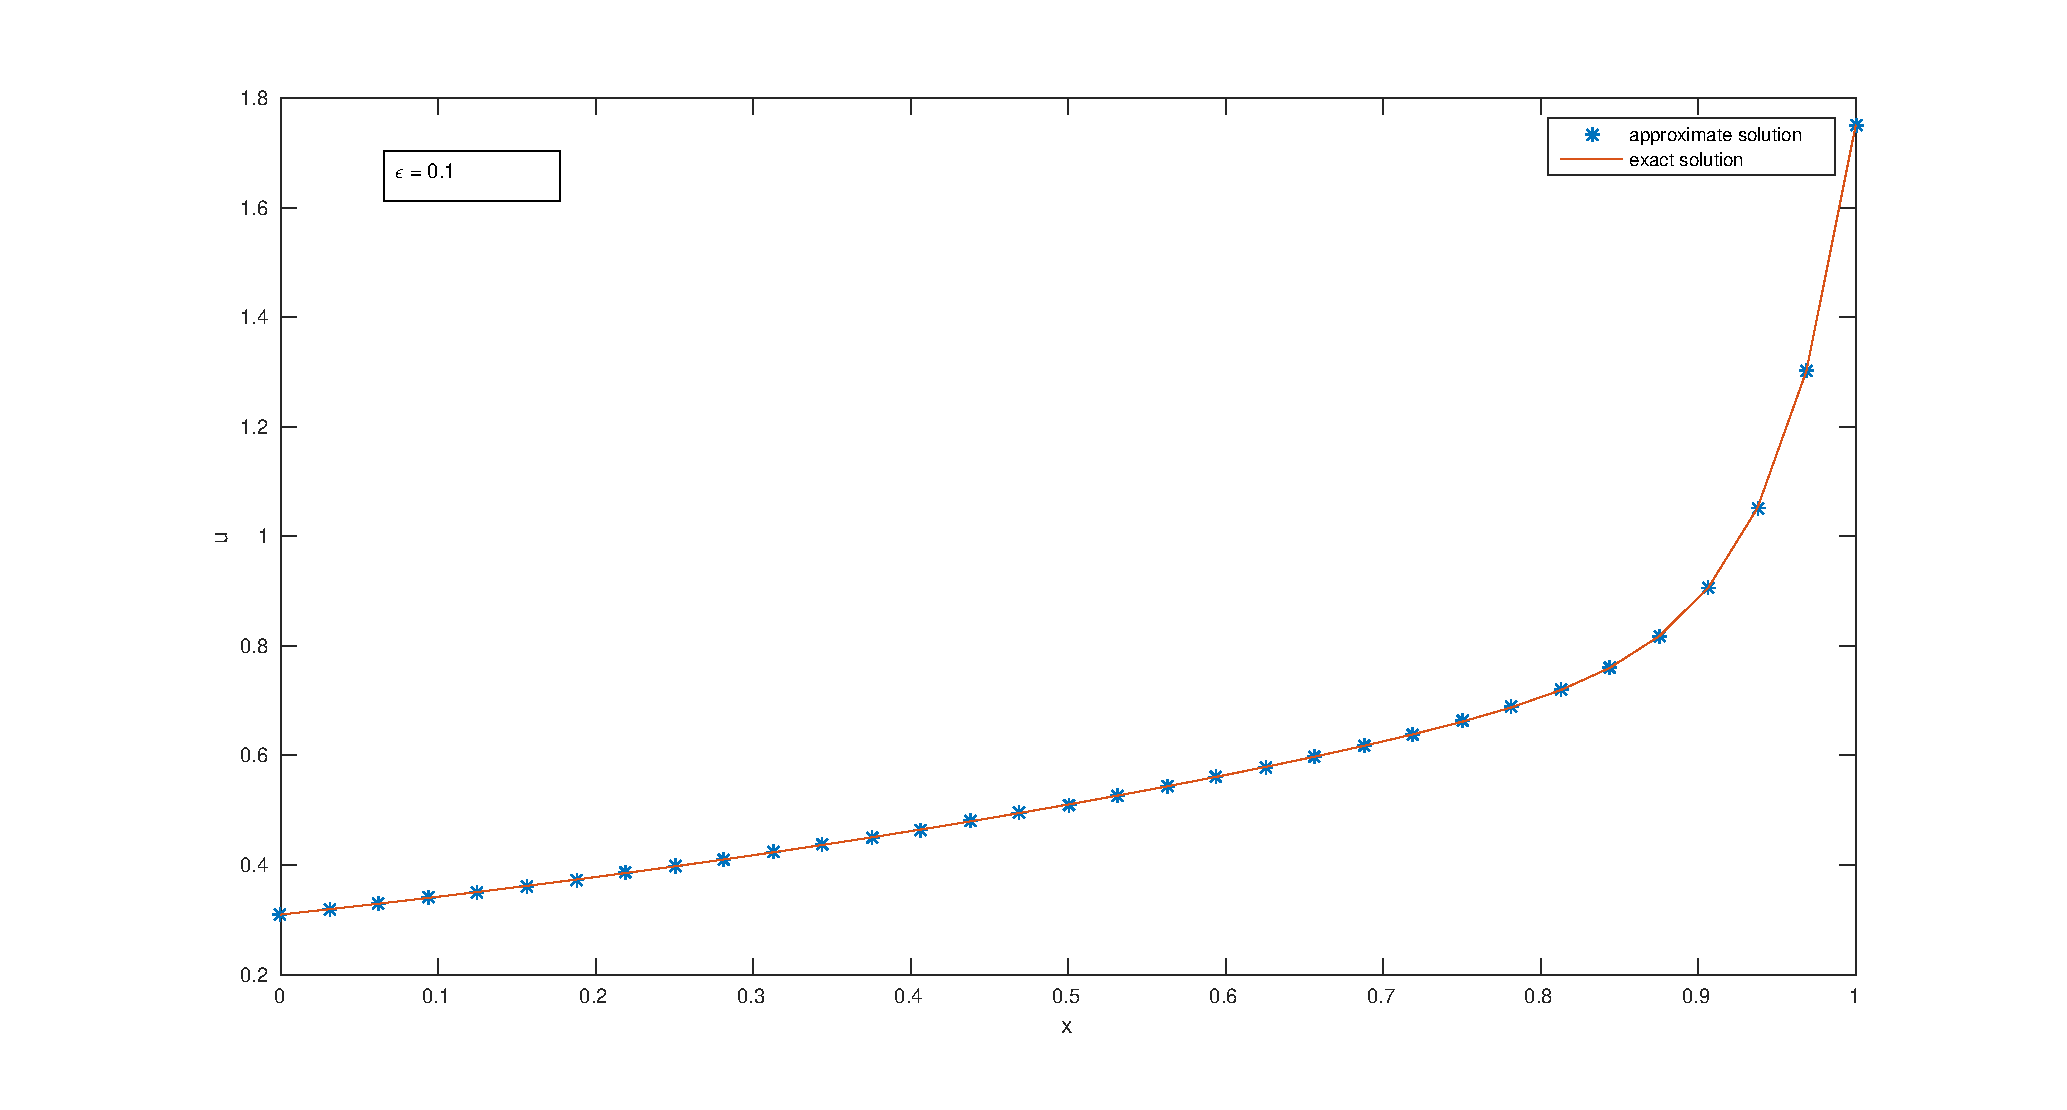
\includegraphics[height=8cm]{Figures/explicit5_2.eps}\\
		\rule{35em}{0.5pt}
	\caption[Parablic]{}
\end{figure}





\chapter{TFPM in two dimensions} % Main chapter title

\label{Chapter3} % For referencing the chapter elsewhere, use \ref{Chapter1} 

\lhead{Chapter 2. \emph{Parabolic and 2D Problem}}

\subsection{Convection-Diffusion-Reaction Problem}

\begin{align}
\mathbb{L}u & \equiv  -\epsilon^{2} \Delta u + p(\textbf{x})u_{x} + q(\textbf{x})u_{y} + b(\textbf{x})u = f(x), \forall \textbf{x} = (x,y) \in \Omega\\
u \large{|}_{\partial{\Omega}} & = 0
\end{align}

For the sake of simplicity, we assume that $\Omega = [0,1] \times [0,1]$ and we have a uniform mesh, i.e
$h = N^{-1}$ be the mesh size and 
\begin{align}
 x_{i} = ih, y_{j} = jh, 0 \leq i , j \leq N
\end{align}

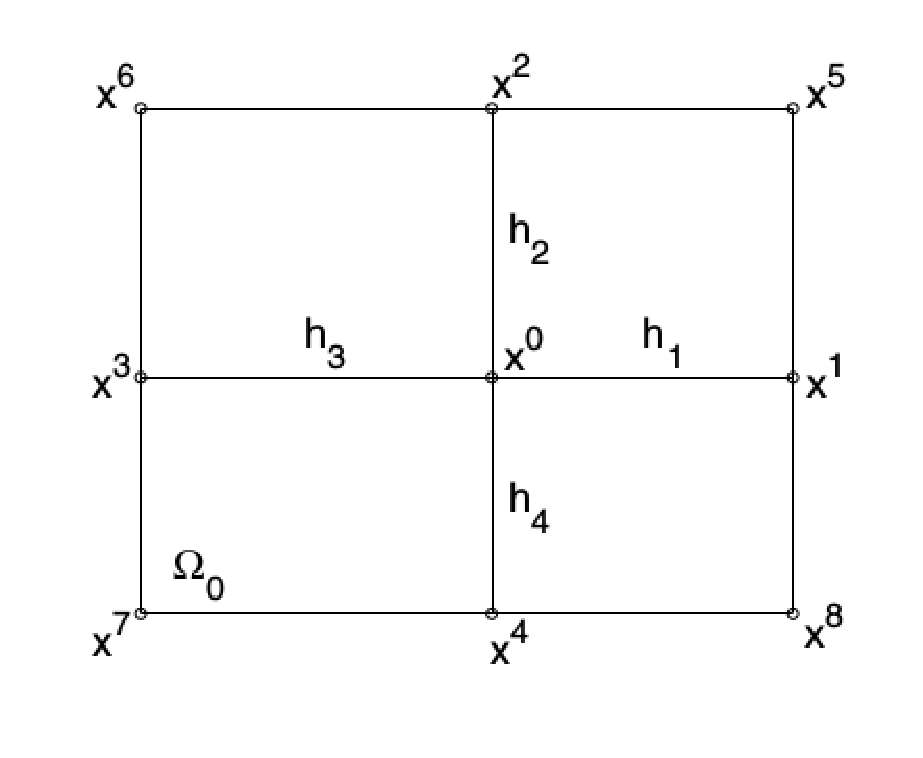
\includegraphics[width =8cm,height = 5cm]{Figures/cell_1.eps}

Then $\{ P_{i,j} = (x_i , y_j ), \hspace{0.3cm} 0 \leq i, j \leq N \}$ are the mesh points.
We construct our TFP scheme for (3.1) on the cell $\Omega_{0}$. We approximate the 
problem  on the cell as follows

\begin{align}
 -\epsilon^{2}\Delta+p_{0}(x)u_{x} + q_{0}u_{y} + b_{0}u = f_{0}
\end{align}
with $p_{0} = p(\textbf{x}^{0}),\hspace{1mm} q_{0} = q(\textbf{x}^{0}),\hspace{1mm} b_{0} = b(\textbf{x}^{0}),\hspace{1mm} f_{0} = f(\textbf{x}^{0})$\\

We consider the case $ b_{0}>0$

Let
\begin{align}
 u(x,y) = \frac{f_{0}}{b_{0}} + v(x,y)\text{exp} \Bigg{(}\frac{p_{0}x + q_{0}y}{2 \epsilon^2}\Bigg{)}
\end{align}
Then we have,

\begin{align}
 -\epsilon^{2} \Delta{v} + d^{2}_{0} = 0
\end{align}

with $d^{2}_{0} = b_{0} + \frac{p_{0}^{2}+q_{0}^{2}}{4 \epsilon^2} $\\
Let $\mu_{0} = d_{0}/\epsilon$, and

\begin{align*}
 H_{4} = \bigg{\{} v(x,y)|\hspace{2mm}v =  c_{1}e^{-\mu_{0}x} + c_{2}e^{\mu_{0}x} + c_{3}e^{-\mu_{0}y} + c_{4}e^{-\mu_{0}y},\hspace{3mm} \forall c_{i} \in \mathbb{R} \bigg{\}}
\end{align*}
Then we take the scheme as

\begin{align}
 \alpha_{1}V_{1} + \alpha_{2}V_{2} + \alpha_{3}V_{3} + \alpha_{4}V_{4} + \alpha_{0}V_{0} = 0
\end{align}
with $V_{j} = v(\textbf{x}^{j})$. Thus we obtain
\begin{align}
 \alpha_{1}e^{-\mu_{0}h} + \alpha_{2} + \alpha_{3}e^{\mu_{0}h} + \alpha_{4}+\alpha_{0} &= 0\\
 \alpha_{1}e^{\mu_{0}h} + \alpha_{2} + \alpha_{3}e^{-\mu_{0}h} + \alpha_{4}+\alpha_{0}&= 0\\
 \alpha_{1} + \alpha_{2}e^{-\mu_{0}h} + \alpha_{3} + \alpha_{4}e^{\mu_{0}h}+\alpha_{0}&= 0\\
 \alpha_{1} + \alpha_{2}e^{\mu_{0}h} + \alpha_{3} + \alpha_{4}e^{-\mu_{0}h}+\alpha_{0} &= 0
\end{align}
For any constant $\alpha_{0} \in \mathbb{R}$ the system (1.10) to (1.13) has the unique solution

\begin{align}
 \alpha_{1} = \alpha_{2} = \alpha_{3} = \alpha_{4} = \frac{-\alpha_{0} }{e^{\mu_{0}h}+e^{-\mu_{0}h}+2} \equiv \frac{-\alpha_{0}}{4\cosh^2\bigg{(}\frac{\mu_{0}h}{2}\bigg{)}}     
\end{align}

On taking

\begin{align}
 \alpha_{0} = \frac{e^{\mu_{0}h}+e^{-\mu_{0}h}+2}{e^{\mu_{0}h}+e^{-\mu_{0}h}-2} \equiv \frac{\cosh^2\bigg{(}\frac{\mu_{0}h}{2}\bigg{)}}{\sinh^2\bigg{(}\frac{\mu_{0}h}{2}\bigg{)}}
\end{align}

we have

\begin{align}
 \alpha_{1} = \alpha_{2}=\alpha_{3} = \alpha_{4} = -\frac{1}{e^{\mu_{0}h}+e^{-\mu_{0}h}+2} \equiv - \frac{1}{4 sinh^{2}\bigg{(}\frac{\mu_{0}h}{2}\bigg{)}}
\end{align}

We ultimately get the following scheme
\begin{align}
 \begin{split}
  U_{0} -& \frac{e^{-\frac{p_{0}h}{2\epsilon^2}}U_{1}+e^{-\frac{q_{0}h}{2\epsilon^2}}U_{2}+e^{\frac{p_{0}h}{2\epsilon^2}}U_{3}+e^{\frac{q_{0}h}{2\epsilon^2}}U_{4}}
  {4cosh^2\bigg{(}\frac{\mu_{0}h}{2}\bigg{)}}\\
  =& \frac{f_{0}}{b_{0}}\Bigg{(}1-\frac{e^{-\frac{p_{0}h}{2\epsilon^2}}+e^{-\frac{q_{0}h}{2\epsilon^2}}+e^{\frac{p_{0}h}{2\epsilon^2}}+e^{\frac{q_{0}h}{2\epsilon^2}}}
  {4cosh^2\bigg{(}\frac{\mu_{0}h}{2}\bigg{)}}\Bigg{)}
 \end{split}
\end{align}
with
\begin{align}
U_{j} = u(\textbf{x}^{j}) = \frac{f_{0}}{b_{0}} + V_{j}\text{exp}\Bigg{(} \frac{p_{0}x + q_{0}y}{2 \epsilon ^2} \Bigg{)}
\end{align}

\subsection{Example}
Consider the following convection-diffusiion-reaction problem along with the given conditions
\begin{align}
 -\epsilon^{2}\Delta u &+ p(\textbf{x})u_{x} + q(\textbf{x})+u_{y}+b(\textbf{x})u = f(\textbf{x}),\hspace{0.5cm} \forall x = (x,y) \in \Omega\\
 u|_{\partial{\Omega}} &= 0
\end{align}
where
\begin{align*}
 &\Omega = [0,1]^2,\hspace{2mm} p(\textbf{x}) = 1,\hspace{2mm} q(\textbf{x}=0),\hspace{2mm} b(\textbf{x}) = 1,\\
 &f(x,y) = [2\epsilon^2 + y(1-y)]\bigg{[}e^{\frac{x-1}{\epsilon^2}} + (x-1)e^{-\frac{1}{\epsilon^2}-x} -x\bigg{]} + y(1-y)\big{(}e^{-\frac{1}{\epsilon^2}}-1\big{)}
\end{align*}
The exact solution of the problem is given by
\begin{align*}
 u(x,y) = y(1-y)\bigg{[}e^{\frac{x-1}{\epsilon^2}} + (x-1)e^{-\frac{1}{\epsilon^2}} -x \bigg{]} 
\end{align*}

The following plots and error estimates have been obtained on solving the above example using the 
tailored finite point method.
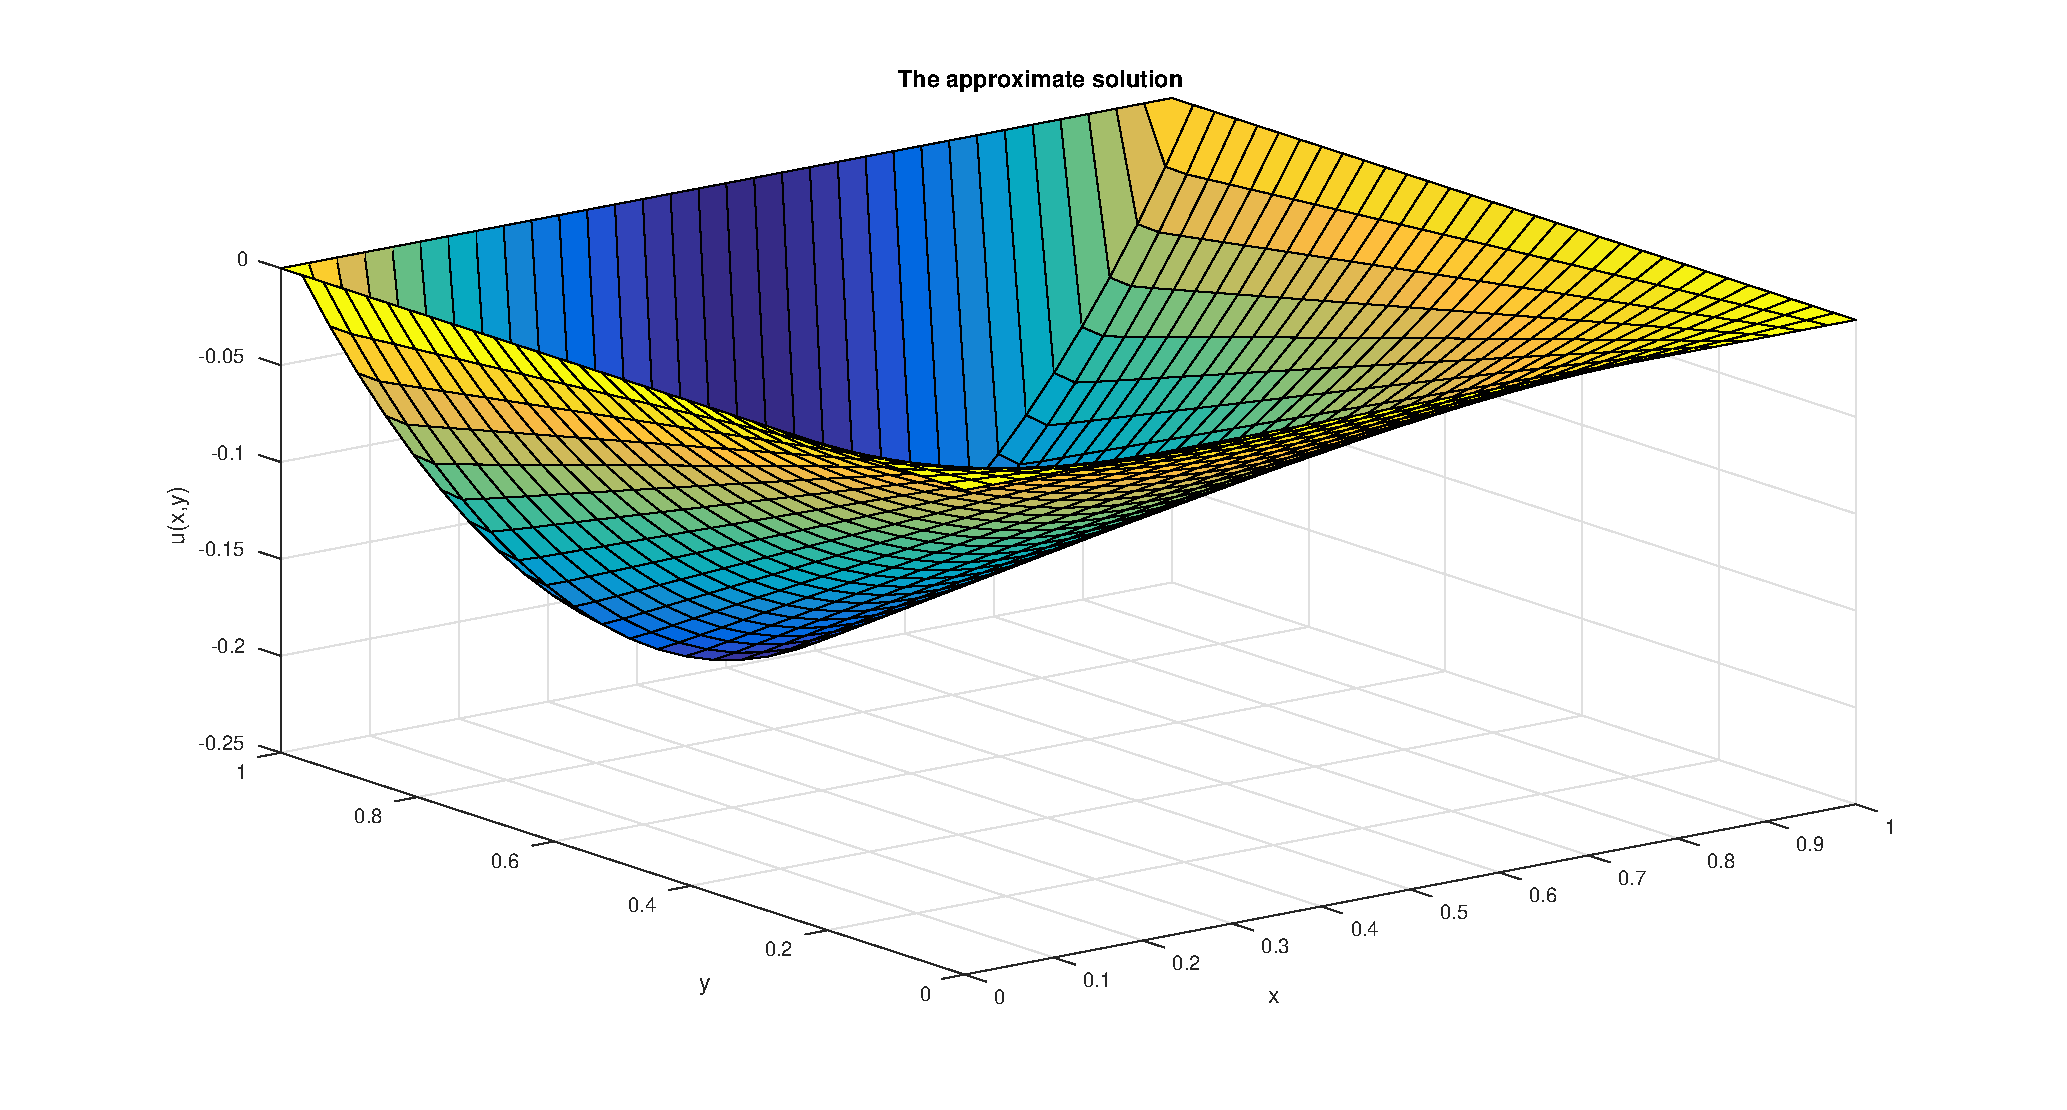
\includegraphics[height=8cm]{Figures/CDR_approx_2.eps}\\
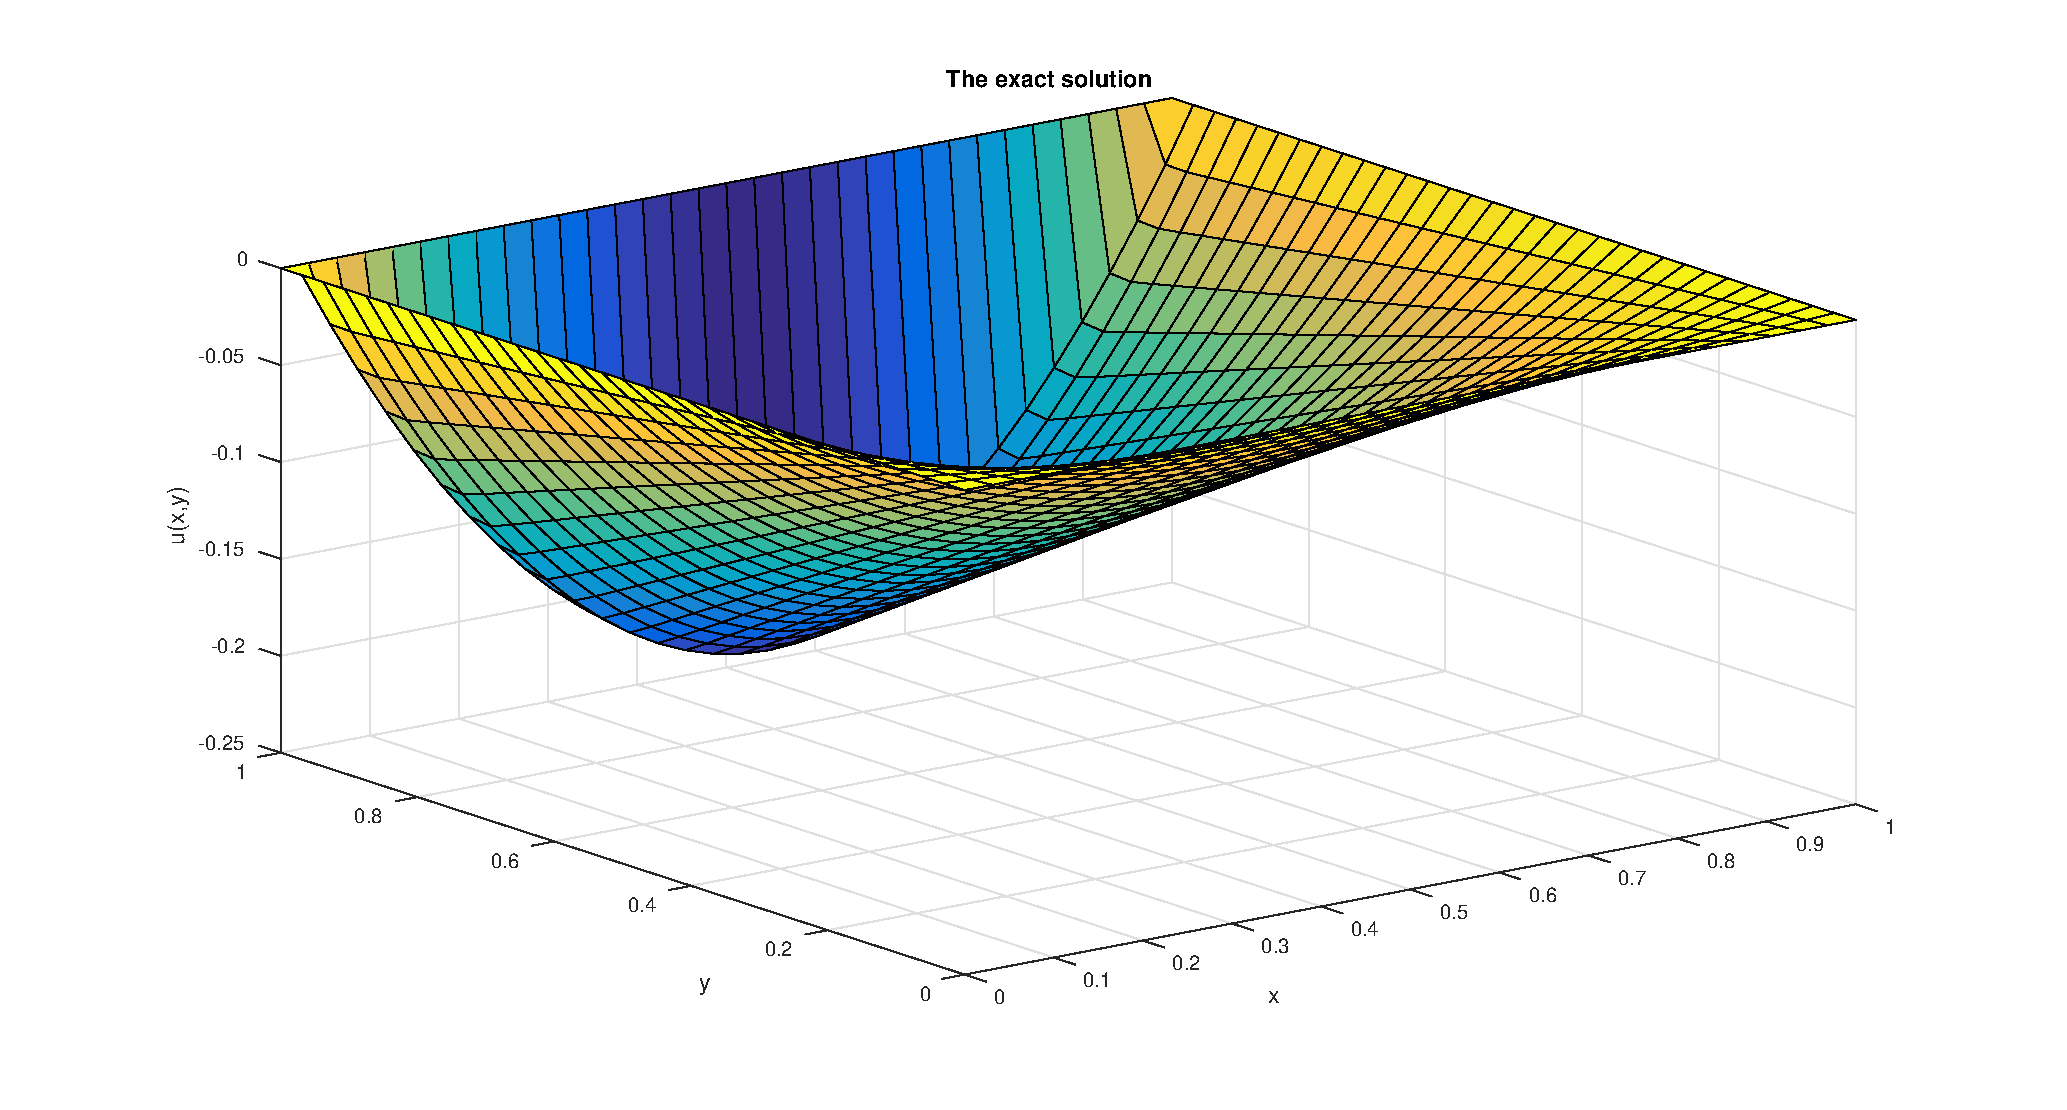
\includegraphics[height=8cm]{Figures/CDR_exact_1.eps}\\

\begin{tabular}{|c|c|c|c|c|c|}
   \hline
  & mesh size h  & 1/16  & 1/32 & 1/64 &  1/128\\
  \hline
 $\epsilon = 0.1$ & Error  & 0.0082  & 0.0032 & 9.4071e-04 &  2.2276e-04\\
 \hline
   &Order & -  &  1.3576  & 1.7662 & 2.0783\\
\hline
  $\epsilon = 0.05$ & Error  & 0.0061  & 0.0038 & 0.0021 &  8.400e-04\\
 \hline
   &Order & -  &  0.6828 & 0.8556 & 1.32\\
\hline
  $\epsilon = 0.01$ & Error  & 0.0048  & 0.0025 & 0.0013 &  6.7100e-04\\
 \hline
   &Order & -  &  0.9411  & 0.9434 & 0.9541\\
\hline
\end{tabular}



\chapter{PCTFPM and Shishkin Mesh Theory}

\label{Chapter3} % For referencing the chapter elsewhere, use \ref{Chapter1} 

\lhead{Chapter 3. \emph{PCTFPM and Shishkin Mesh}}

The theory of some other concepts/methods which were encountered during the course of this thesis is described here.

\section{Parallelogram Centred Tailored Finite Point Method (PCTFPM)}

\begin{figure}[htbp]
	\centering
		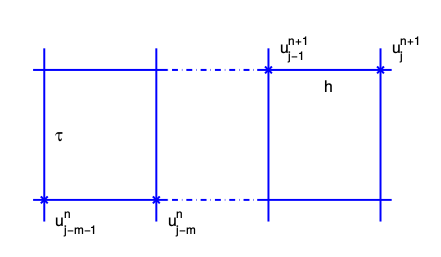
\includegraphics[height=4cm]{Figures/mesh_PCTFPM.png}\\
	\caption[RCTFPM imaginary part]{}
\end{figure}
The parallelogram scheme is given as follows:
\begin{align*}
 u_{j}^{n+1} = \alpha_{-1}u_{j-1}^{n+1}+\beta_{-1}u_{j-m-1}^{n}+\beta_{0}u_{j-m}^{n}
\end{align*}

As seen from the mesh and from the scheme, there is a diagonal like correspondance between the points of the next time step and the current
time step. This can be useful whenever there is a discontinuity in the initial condition or an interior layer is being formed because 
of a discontinuous source term or a discontinuous coefficient.

By using the basis
\begin{align*}
 V = {\{} v(x,t)|v(x,t) =  c_{1} + c_{2}e^{(ik_{j}(at-x))} + c_{3}e^{-(ik_{j}(at-x))}, \hspace{0.5cm} \forall c_{1}, c_{2}, c_{3} \in \mathbb{C} {\}}  
\end{align*}

Taking the coeffecients $(c_1, c_2, c_3)$ as (1,0,0), (0,1,0), (0,0,1) we get
\begin{align*}
 1 &= \alpha_{-1} + \beta_{-1} + \beta_{0} \\
 cos(k_{j}a \tau ) &= \alpha_{-1}\cos(k_{j}(a \tau + h)) + \beta_{-1}\cos(k_{j}(m+1)h) + \beta_{0}\cos(mh)\\
 sin(k_{j}a \tau ) &= \alpha_{-1}\sin(k_{j}(a \tau + h)) + \beta_{-1}\sin(k_{j}(m+1)h) + \beta_{0}\sin(mh)
\end{align*}

Thus we get

\begin{align*}
 \alpha_{-1} &= \frac{\sin(k_{j}(a \tau -(m+1)h)/2)}{\sin(k_{j}(a \tau -(m-1)h)/2)}\\
 \beta_{-1} &= 1\\
 \beta_{0} &= -\alpha_{-1}
\end{align*}

PCTFPM is unconditionally stable and has second order convergence in space.


\section{Shishkin Mesh}

An approach to solving parabolic problem on a Shishkin mesh is described here.

The problem is as follows:

\begin{align*}
 &u_{t} - \epsilon u_{xx} + b u_{x} = 0 \text{ for } (x,t) \in \Omega = (0,1)\\
 &u(x,0) = \phi(x)\\
 &u(0,t) = \alpha(t), \hspace{5mm} u(1,t) = \beta(t)
\end{align*}

\begin{figure}[htbp]
	\centering
		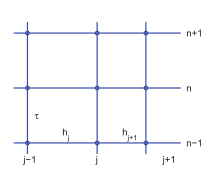
\includegraphics[height=4cm]{Figures/shiskin.png}\\
	\caption[RCTFPM imaginary part]{}
\end{figure}

\subsection{Construction of the mesh and an Implicit Scheme}
We consider the interval $[0,1]$. Let $\sigma = \max\{\frac{1}{2},1-\frac{2 \epsilon}{b}ln(N)\}$, where N is the number
of intervals in the mesh. The mesh is divided into $[0,\sigma]$ and $[\sigma,1]$ in $(N/2)$ equidistant parts.

\begin{align*}
x_{j} = \begin{cases} 
	    jH \hspace{1cm} \text{when} j \leq N/2\\
	    \sigma + (j-\frac{N}{2})h \hspace{1cm} \text{when} j>N/2\\
	 \end{cases}
\end{align*}

where
\begin{align*}
 H &= \frac{2 \sigma}{N}\\
 h &= \frac{2(1-\sigma)}{N}
\end{align*}

\begin{align*}
 u_{j}^{n} = a_{1}u_{j-1}^{n+1} + a_{2}u_{j}^{n+1} + a_{3}u_{j+1}^{n+1}
\end{align*}

The basis used is

\begin{align*}
 \{ 1, x-bt, e^{\frac{bx}{\epsilon}} \}
\end{align*}

Substituting these basis functions we get

\begin{align*}
 &a_{1}+a_{2}+a_{3} = 1\\
 &a_{1}(-h_{j})+a_{3}h_{j+1} = b \tau\\
 &a_{1}e^{-\frac{bh_{j}}{\epsilon}}+a_{2}+a_{3}e^{-\frac{bh_{j+1}}{\epsilon}} = 1
\end{align*}

Solving the above system leads to

\begin{align*}
 a_{1} &= \frac{b \tau (e^{bh_{j+1}/\epsilon}-1)}{h_{j+1}(1-e^{-bh_{j}/\epsilon}) - h_{j}(e^{bh_{j+1}/\epsilon}-1)}\\
 a_{3} &= \frac{b \tau (1-e^{-bh_{j}/\epsilon})}{h_{j+1}(1-e^{-bh_{j}/\epsilon}) - h_{j}(e^{bh_{j+1}/\epsilon}-1)}\\
 a_{2} &= 1-a_1-a_3
\end{align*}

Thus the above scheme can be used to solve parabolic problems on a Shishkin mesh.

% Chapter 1

\chapter*{References} % Main chapter title

%\label{Chapter3} % For referencing the chapter elsewhere, use \ref{Chapter1} 

\begin{enumerate}
 \item Houde Han, Zhongyi Huang, and R. Bruce Kellogg, A tailored finite point method for a
singular perturbation problem on an unbounded domain, J. Sci. Comput. 36 (2008), no. 2,
243-261.
\item Han, H., Huang, Z.Y.: Tailored finite point method based on exponential bases for
convection-diffusion-reaction equation. Math. Comput. 82, 213-226 (2013).
\item Han, H., Huang, Z.Y.: Tailored finite point method for steady-state reaction-diffusion
equation. Commun. Math. Sci. 8, 887-899 (2010)
\item Z. Huang and X. Yang, Tailored finite point method for first order wave equation, Journal of
Scientific Computing, 49 (2011), 351-366.
\item Huang, Z. and Yang, Y. (2016). Tailored Finite Point Method for Parabolic Problems. Computational Methods in Applied Mathematics, 
16(4), pp. 543-562.
\end{enumerate}

%----------------------------------------------------------------------------------------



%\input{Chapters/Chapter6}
%\input{Chapters/Chapter7}

%-------------------------------------------------------------------------------
%	THESIS CONTENT - APPENDICES
%-------------------------------------------------------------------------------
\addcontentsline{toc}{chapter}{Referencesth}
\addtocontents{toc}{\vspace{2em}} % Add a gap in the Contents, for aesthetics

%\appendix % Cue to tell LaTeX that the following 'chapters' are Appendices

% Include the appendices of the thesis as separate files from the Appendices
% folder
% Uncomment the lines as you write the Appendices

%% Appendix A

\chapter{Appendix Title Here} % Main appendix title

\label{AppendixA} % For referencing this appendix elsewhere, use \ref{AppendixA}

\lhead{Appendix A. \emph{Appendix Title Here}} % This is for the header on each page - perhaps a shortened title

Write your Appendix content here.
%\input{Appendices/AppendixB}
%\input{Appendices/AppendixC}

\addtocontents{toc}{\vspace{2em}} % Add a gap in the Contents, for aesthetics
\backmatter

%-------------------------------------------------------------------------------
%	BIBLIOGRAPHY
%-------------------------------------------------------------------------------

\label{Bibliography}

\lhead{\emph{Bibliography}} % Change the page header to say "Bibliography"

%\printbibliography

\end{document}
